%==========================================================================
% Where the Policy Ends and the User Begins:
%   A Boundary-Case Mismatch in App-Store Privacy Labels
% Manuscript for submission to:
%   International Journal of Human-Computer Studies (Elsevier)
%
% Build:   pdflatex main && bibtex main && pdflatex main && pdflatex main
%==========================================================================
\documentclass[11pt,a4paper]{article}

\usepackage[T1]{fontenc}
\usepackage[utf8]{inputenc}
\usepackage{lmodern}
\usepackage{microtype}
\usepackage[a4paper,margin=2.3cm]{geometry}
\usepackage{lineno}
\usepackage{amsmath,amssymb}
\usepackage{booktabs,array,multirow,makecell}
\usepackage{xcolor}
\usepackage{graphicx}
\usepackage{natbib}
\bibliographystyle{plainnat}
\usepackage{hyperref}
\hypersetup{colorlinks=true, linkcolor=blue!55!black,
            citecolor=teal!60!black, urlcolor=blue!55!black}
\usepackage{placeins}
\usepackage{fancyhdr}
\pagestyle{fancy}
\fancyhf{}
\fancyhead[L]{\small\itshape Where the Policy Ends and the User Begins}
\fancyhead[R]{\small\itshape Submitted to Int. J. of Human--Computer Studies}
\fancyfoot[C]{\small\thepage}
\renewcommand{\headrulewidth}{0.4pt}
\renewcommand{\footrulewidth}{0pt}
\makeatletter
\let\@oldsection\section
\renewcommand{\section}{\FloatBarrier\@oldsection}
\makeatother
\renewcommand{\topfraction}{0.95}
\renewcommand{\bottomfraction}{0.7}
\renewcommand{\textfraction}{0.05}
\renewcommand{\floatpagefraction}{0.7}
\setcounter{topnumber}{4}
\setcounter{bottomnumber}{2}
\setcounter{totalnumber}{6}

% TikZ / pgfplots
\usepackage{tikz}
\usepackage{pgfplots}
\pgfplotsset{compat=1.18}
\usetikzlibrary{arrows.meta, positioning, fit, calc,
                shapes.geometric, shapes.symbols, shadows.blur,
                decorations.pathmorphing, backgrounds, patterns,
                matrix, decorations.markings}

% ===== Palette =====
\definecolor{bmGreen}{RGB}{46,160,67}
\definecolor{bmAmber}{RGB}{240,160,40}
\definecolor{bmRed}{RGB}{214,39,40}
\definecolor{bmBlue}{RGB}{31,119,180}
\definecolor{bmPurple}{RGB}{148,103,189}
\definecolor{bmTeal}{RGB}{23,190,207}
\definecolor{bmInk}{RGB}{55,65,81}
\definecolor{bmSlate}{RGB}{73,80,87}
\definecolor{bmCream}{RGB}{252,247,234}
\definecolor{bmPink}{RGB}{227,119,194}
\definecolor{bmGold}{RGB}{241,196,15}

\definecolor{tierPolicy}{RGB}{27,94,32}
\definecolor{tierLabel}{RGB}{255,143,0}
\definecolor{tierUser}{RGB}{183,28,28}
\definecolor{tierMid}{RGB}{55,71,79}

\linenumbers

\title{\textbf{Where the Policy Ends and the User Begins:\\
A Boundary-Case Mismatch in App-Store Privacy Labels}\\[4pt]
\large \textit{Submitted to International Journal of Human-Computer Studies}}
\author{Anonymous Author(s)\\\small Anonymised for review}
\date{}

\begin{document}
\maketitle

%==========================================================================
% IJHCS REQUIRED: Highlights (3--5 bullet points, each $\leq$ 85 chars).
% Submitted as a separate file at production; reproduced here for review.
%==========================================================================
\begin{center}
\fbox{\begin{minipage}{0.94\linewidth}
\textbf{Highlights}\smallskip
\begin{itemize}\setlength\itemsep{1pt}\small
\item App-store privacy labels run 9 hidden \emph{boundary cases}
      before showing any flag.
\item 87-user survey measures per-case agreement on Google Play's nine
      boundary cases.
\item Maybe-rate exceeds 16\% on every case; off-device-ephemeral hits
      38.2\% Maybe.
\item We name the gap the \emph{boundary-case mismatch}; label accuracy is
      two-layer, not one.
\item Boundary-Layer Explainer pattern: rule clause + community signal +
      one-tap toggle.
\end{itemize}
\end{minipage}}
\end{center}
\vspace{4pt}

\begin{abstract}\normalsize
App-store privacy labels report \emph{collection} and \emph{sharing}
as binary flags. Each flag, however, is the output of a hidden chain
of policy \emph{boundary cases} that decide what counts as collection
or sharing in the first place. We surveyed 87 Android users on Google
Play's nine boundary cases (on-device, end-to-end encryption,
off-device ephemeral, redirect, user-initiated, prominent consent,
service-provider, legal, anonymised) and measured per-case agreement
with the platform's interpretation. Yes-rates range from $61.8\%$
(off-device ephemeral) to $83.3\%$ (end-to-end encryption); the
\emph{Maybe} rate exceeds $16\%$ on every case and reaches $38.2\%$
on off-device ephemeral processing and $28.4\%$ on anonymised
transfer --- the two cases where the policy claim is hardest to
verify. We name this gap the \emph{boundary-case mismatch} and
argue that label accuracy has two layers: \emph{policy alignment}
(does the flag follow from the practice under policy?) and
\emph{user alignment} (would the user issue the same flag?). The
literature has audited the first; this paper measures the second.
We contribute (i) a two-layer accuracy framework, (ii) a first
per-boundary-case empirical baseline at the user-alignment layer,
and (iii) a falsifiable design pattern --- the
\emph{Boundary-Layer Explainer} --- that surfaces the inference rule
in user-side language. A pre-registered mixed-method evaluation of
the pattern (online vignette experiment plus think-aloud sessions)
is described in Section~\ref{sec:eval-plan}; the present paper
reports the measurement contribution. Limitations include a modest
crowd-work sample and the absence of a deployed redesign study.
\end{abstract}

\noindent\textbf{Keywords:} privacy labels; Data Safety;
Google Play; boundary cases; legal-technical alignment;
usable privacy; mental models; HCI.

%==========================================================================
\section{Introduction}\label{sec:intro}

A privacy label is an output. The flag ``\textsc{shares Location with
third parties}'' in Google Play's Data Safety section is the visible
endpoint of a chain of policy decisions made silently before it
reached the user. Is the recipient a \emph{service provider} acting
on the developer's behalf? Is the transfer \emph{user-initiated} in a
way the user could reasonably expect? Is the data \emph{anonymised}
so it can no longer be linked to an individual? Has consent been
collected ``in a way that meets the requirements of Google Play's
User Data policy''~\citep{google:data:safety:2022}? Each link in this
chain is a \emph{boundary case}: a policy rule that converts a
practice into either ``does count'' or ``does not count'' as
collection or sharing for disclosure purposes. The user sees only the
final binary flag. The boundary cases that produced it are not
surfaced.

Two decades of usable-privacy research have asked whether users
\emph{understand} the categories and purposes that appear inside a
label~\citep{kelley:etal:2009,kelley:etal:2010,kelley:etal:2013,
zhang:etal:2022,reidenberg:etal:2015}. A parallel literature has
asked whether labels are \emph{honest}, auditing the gap between what
an app declares and what an app does~\citep{koch:etal:2022,
kollnig:etal:2022,bhagavatula:etal:2023,khandelwal:etal:2023,
andow:etal:2020}. Both are about the contents of the label. The
question we raise is one step earlier in the pipeline. \emph{Before}
a flag can be honest or comprehensible, a policy rule has to decide
what the flag should be. That rule has a policy answer. It also has a
user answer. \textbf{The boundary-case mismatch is the gap between
the two.}

% -----------------------------------------------------------------
% Figure 1: The disclosure pipeline (Practice -> Boundary set -> Flag -> User).
% Compact layout, fits \linewidth without aggressive resize.
% -----------------------------------------------------------------
\begin{figure}[!htbp]
\centering
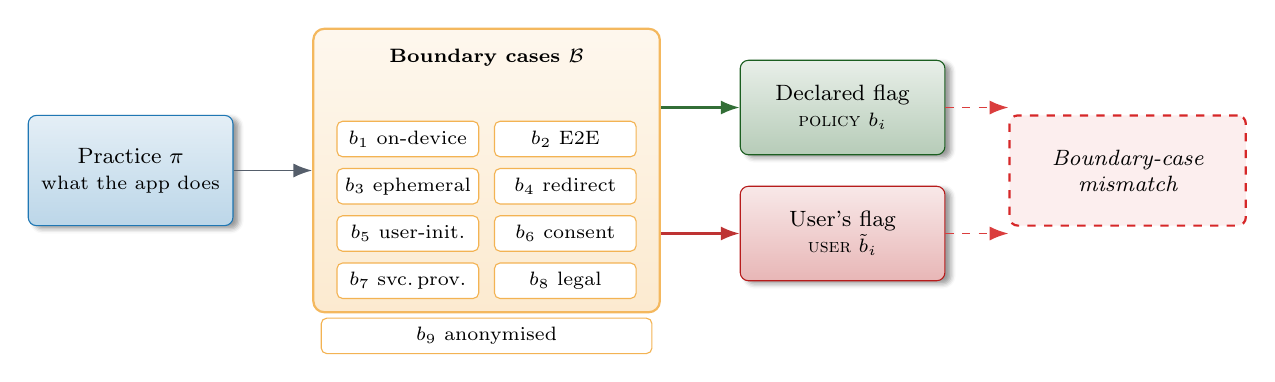
\begin{tikzpicture}[font=\sffamily,
  box/.style={draw=bmInk!80,rounded corners=3pt,minimum width=23mm,
              minimum height=12mm,align=center,font=\footnotesize,
              blur shadow={shadow blur steps=4,shadow yshift=-0.4mm}},
  practice/.style={box,top color=bmBlue!12,bottom color=bmBlue!30,draw=bmBlue,
                   minimum width=26mm,minimum height=14mm},
  bgroup/.style={draw=bmAmber!75,thick,rounded corners=4pt,
                 top color=bmAmber!8,bottom color=bmAmber!22,
                 minimum width=44mm,minimum height=36mm,align=center,
                 font=\footnotesize\itshape\bfseries,inner sep=0pt},
  bcase/.style={draw=bmAmber!80,rounded corners=2pt,fill=white,
                font=\scriptsize,minimum width=18mm,minimum height=4.5mm,
                inner sep=1.5pt,align=center},
  policy/.style={box,top color=tierPolicy!10,bottom color=tierPolicy!32,
                 draw=tierPolicy,minimum width=26mm,minimum height=12mm},
  user/.style={box,top color=tierUser!10,bottom color=tierUser!32,
               draw=tierUser,minimum width=26mm,minimum height=12mm},
  mm/.style={draw=bmRed,thick,dashed,rounded corners=3pt,fill=bmRed!8,
             font=\footnotesize\itshape,align=center,
             minimum width=30mm,minimum height=14mm},
  arr/.style={-{Latex[length=2.4mm]},line width=0.7pt,draw=bmInk!85}]

% Practice (left)
\node[practice] (pi) at (0,0) {Practice $\pi$\\ \scriptsize what the app does};

% Boundary group (center) with internal cases
\node[bgroup,right=10mm of pi] (B) {};
\node[font=\scriptsize\bfseries,anchor=north] at ($(B.north)+(0,-1.5mm)$)
   {Boundary cases $\mathcal{B}$};
\foreach \i/\name/\x/\y in {%
  1/{$b_1$ on-device}/-10mm/4mm,
  2/{$b_2$ E2E}/10mm/4mm,
  3/{$b_3$ ephemeral}/-10mm/-2mm,
  4/{$b_4$ redirect}/10mm/-2mm,
  5/{$b_5$ user-init.}/-10mm/-8mm,
  6/{$b_6$ consent}/10mm/-8mm,
  7/{$b_7$ svc.\,prov.}/-10mm/-14mm}
   \node[bcase] at ($(B.center)+(\x,\y)$) {\name};
\node[bcase,minimum width=18mm] at ($(B.center)+(10mm,-14mm)$) {$b_8$ legal};
\node[bcase,minimum width=42mm] at ($(B.center)+(0mm,-21mm)$) {$b_9$ anonymised};

% Right column: two flags
\node[policy,right=10mm of B,yshift=8mm]  (flag) {Declared flag\\ \scriptsize \textsc{policy} $b_i$};
\node[user,right=10mm of B,yshift=-8mm]   (uflag) {User's flag\\ \scriptsize \textsc{user} $\tilde b_i$};

% Mismatch
\node[mm,right=8mm of flag,yshift=-8mm] (mmnode) {Boundary-case\\ mismatch};

% Arrows
\draw[arr] (pi.east) -- (B.west);
\draw[arr,draw=tierPolicy!90,thick] (B.east |- flag) -- (flag.west);
\draw[arr,draw=tierUser!90,thick]   (B.east |- uflag) -- (uflag.west);
\draw[arr,draw=bmRed!90,dashed] (flag.east) -- (mmnode.west |- flag);
\draw[arr,draw=bmRed!90,dashed] (uflag.east) -- (mmnode.west |- uflag);
\end{tikzpicture}
\caption{The disclosure pipeline. Each data-handling practice $\pi$
passes through the set $\mathcal{B}$ of nine policy boundary cases.
The platform applies the predicates $b_i$ to produce the declared
flag; the user applies their own predicates $\tilde b_i$ to form a
private user-side flag. When the two disagree, the result is a
\emph{boundary-case mismatch}: a flag that is accurate under policy
and wrong under the user's own theory of what the words mean.}
\label{fig:pipeline}
\end{figure}


Figure~\ref{fig:pipeline} expands the picture. A data-handling
practice $\pi$ is reported as collection or sharing only if none of
the boundary-case exceptions apply. Each exception is itself a small
inferential boundary --- e.g., ``off-device processing without
retention is not collection''. The policy reads this disjunction as a
Boolean partition; the user must, separately, decide whether they
agree that the practice falls on the policy's side of the line.
\emph{The same flag can be ``accurate'' to the policy and ``wrong''
to the user when policy and user place the boundary in different
places.}

This paper has three contributions:

\textbf{(1) A measurement framework.} We argue label correctness
cannot be reduced to either auditing the declaration or testing user
comprehension. It must additionally be measured at the level of the
\emph{boundary inferences} that produced the declared flag. We
formalise this as a two-layer definition (Sec.~\ref{sec:framework}):
\emph{policy-layer accuracy} (does the flag follow from policy given
the practice?), and \emph{user-layer accuracy} (does the user, given
the same practice, issue the same flag?).

\textbf{(2) A per-boundary-case empirical baseline.}
We survey 87 Android users about each of Google Play's nine boundary
cases and report Yes / Maybe / No distributions with Wilson 95\%
confidence intervals. Agreement ranges from $61.8\%$ to $83.3\%$;
the \emph{Maybe} rate is concentrated on the cases most implicated
in the ``does it count?'' debate, reaching $38.2\%$ on off-device
ephemeral processing and $28.4\%$ on anonymised transfer.

\textbf{(3) A design pattern.}
We propose \emph{Boundary-Layer Explainers} (BLEs): plain-language
renderings of the specific exception that produced the visible flag,
expressed in the user's own consequence-first language (\emph{Does
the data leave the device? Who can access it? How long is it kept?
Can it be linked back to me?}). We present BLE patterns for the
widest-gap cases, a worked mock-up, and an architectural sketch.

The paper is organised as follows. Section~\ref{sec:related} situates
the contribution against the privacy-label, mental-models, and
contextual-integrity literatures. Section~\ref{sec:framework}
develops the two-layer accuracy framework.
Section~\ref{sec:method} reports the method and corpus.
Section~\ref{sec:results} presents results across the four parts of
the instrument. Section~\ref{sec:mismatch} synthesises the
boundary-case mismatch typology and the BLE design pattern.
Section~\ref{sec:discussion} discusses implications and limitations.
Section~\ref{sec:conclusion} concludes.

%==========================================================================
\section{Background and Related Work}\label{sec:related}

We draw on four literatures: nutrition-style privacy labels and their
user-side evaluation; mental models of mobile privacy; contextual
integrity as a theory of appropriate flow; and audit work on the
declared-vs-observed honesty of app-store labels. Our contribution
sits at their intersection: the \emph{inference layer} the four
literatures assume but rarely measure.

\paragraph{Nutrition-label privacy disclosures.}
The cost of reading a website privacy policy was estimated at
\textit{ca.}\ 244 hours per user per
year~\citep{mcdonald:cranor:2008,solove:2013,cranor:2012}. The
``nutrition label'' line of work~\citep{kelley:etal:2009,
kelley:etal:2010,kelley:etal:2013,schaub:etal:2015} responded with a
standardised, scannable disclosure: a category $\times$ purpose
matrix that lets users compare data practices across apps. Apple
deployed this idea as the App Privacy Nutrition Label in
December~2020~\citep{apple:label:2020}; Google followed with the Data
Safety section in July~2022~\citep{google:data:safety:2022}. Both
share the same disclosure unit: a binary flag per category, conditioned
by a fixed list of purposes.

\paragraph{Comprehension and recall.}
Usability studies of Apple's labels~\citep{zhang:etal:2022} report
high recall failure rates for specific category language and a
non-negligible share of users who interpret a missing flag as a
guarantee rather than a non-claim. Earlier work on Android
permissions found systematic gaps between what users believe a
permission grants and what it actually grants~\citep{felt:etal:2012,
felt:etal:2012b,liccardi:etal:2014,tan:etal:2014,
wijesekera:etal:2015,wijesekera:etal:2017}. The broader survey
literature on privacy notices reaches the same conclusion: privacy
notices are read shallowly, scanned for absolutes, and reasoned about
with informal heuristics~\citep{jensen:potts:2004,acquisti:etal:2015,
acquisti:etal:2017,adjerid:etal:2013,good:etal:2007,
acquisti:grossklags:2005,brandimarte:etal:2013}. These results
address whether users \emph{recognise} category language; they do not
address whether users agree with the \emph{rule} that turned a
practice into a Yes or a No.

\paragraph{Mental models and folk theories.}
Mental-models studies show that users carry well-developed but
non-technical theories of how data flows through systems~\citep{
wash:2010,wash:rader:2015,kang:etal:2015,lin:etal:2012,
lin:etal:2014,rader:etal:2012,sannon:etal:2018}. Wash's folk-model
taxonomy~\citep{wash:2010} is a paradigmatic example: users do not
hold wrong beliefs, they hold \emph{different} beliefs, organised
into coherent stories. We will see the same in our boundary-case
rationales. Users who reject the ``does not count as collection''
framing typically do so on the grounds that the \emph{capability} to
collect already exists --- a folk-theoretic version of the
privacy-engineering principle that data collection should be assessed
by potential, not by the developer's
intention~\citep{spiekermann:cranor:2009,cavoukian:2009}.

\paragraph{Contextual integrity.}
Contextual integrity~\citep{nissenbaum:2004,nissenbaum:2010,
barth:etal:2006,martin:nissenbaum:2017,apthorpe:etal:2018,
shvartzshnaider:etal:2019} reframes privacy as appropriate flow under
context-specific norms. CI-based studies of mobile
permissions~\citep{wijesekera:etal:2015,wijesekera:etal:2017,
naeini:etal:2017} show that user comfort with the same data flow
varies dramatically across contexts. The Data Safety section, by
collapsing all of an app's flows into a context-free category $\times$
purpose matrix, \emph{cannot represent} the contextual judgments CI
says are constitutive of privacy. The boundary-case layer is where
this collapse occurs.

\paragraph{Audits: is the declared label honest?}
A parallel literature audits whether labels match observed runtime
behaviour. \citet{kollnig:etal:2022} found that iOS App Tracking
Transparency did not in fact reduce tracker presence in apps even
where the label said the app did not track; \citet{koch:etal:2022}
extended the methodology and reported widespread under-declaration.
\citet{bhagavatula:etal:2023} interviewed developers and found that
the declaration process is itself error-prone and under-supported.
\citet{khandelwal:etal:2023} performed the most recent large-scale
audit of Google Play's Data Safety section and reported systematic
under-disclosure, in part because developers themselves disagree with
platform-supplied boundary definitions. Companion work on policy-text
analysis~\citep{wilson:etal:2016,harkous:etal:2018,cui:etal:2023,
andow:etal:2020,reyes:etal:2018,razaghpanah:etal:2018,
englehardt:narayanan:2016,nguyen:etal:2022,ren:etal:2018,
shipp:blasco:2020} shows the same pattern at the policy-text level.
This work measures the policy--label gap; we measure the label--user
gap one step further down the pipeline.

\paragraph{Summary.}
Privacy labels have been studied as comprehension artefacts (do users
read them right?), as honesty artefacts (do developers fill them in
right?), and as design artefacts (can we design them better?). We add
a fourth question: \emph{do users agree that the rule that produced
the visible flag was the right rule to apply?} If they do not --- and
we will show that in nine out of nine boundary cases, a meaningful
fraction does not --- then the label can be honest, recall its
categories perfectly, and still mislead.

%==========================================================================
\section{Conceptual Framework: Two-Layer Label Accuracy}\label{sec:framework}

Let $\pi$ be an observable data practice (e.g., ``sends device IDs to
an SDK''). Let $\mathcal{B}=\{b_1,\ldots,b_9\}$ be Google Play's
boundary cases. Each $b_i$ is a Boolean predicate on
$\pi$: $b_i(\pi)\in\{0,1\}$. Google Play's disclosure rule for a
category $c$ may be written
\begin{equation}\label{eq:policy}
\textrm{flag}_\textsc{policy}(\pi,c) \;=\; \mathbb{1}\!\left[\pi
\text{ affects }c \;\wedge\; \bigwedge_{b_i\in \mathcal{B}_c}
\lnot\, b_i(\pi)\right],
\end{equation}
where $\mathcal{B}_c\subseteq\mathcal{B}$ is the set of boundary
cases the policy authorises as exceptions for category $c$. A
practice is reported only if it affects the category and \emph{no}
authorising exception applies. The user, given the same practice and
the same set of boundary cases, applies their own predicates
$\tilde{b}_i$:
\begin{equation}\label{eq:user}
\textrm{flag}_\textsc{user}(\pi,c) \;=\; \mathbb{1}\!\left[\pi
\text{ affects }c \;\wedge\; \bigwedge_{b_i\in \mathcal{B}_c}
\lnot\, \tilde{b}_i(\pi)\right].
\end{equation}
\textbf{Policy-layer accuracy} is the property that the displayed
flag equals $\textrm{flag}_\textsc{policy}(\pi,c)$ for the actual
$\pi$; this is what existing audits~\citep{koch:etal:2022,
kollnig:etal:2022,khandelwal:etal:2023} measure. \textbf{User-layer
accuracy} is the property that the displayed flag equals
$\textrm{flag}_\textsc{user}(\pi,c)$. The disagreement set is
$\{\pi : \textrm{flag}_\textsc{policy} \neq
\textrm{flag}_\textsc{user}\}$; the \emph{boundary-case mismatch
rate} for $b_i$ is the share of users whose $\tilde{b}_i$ disagrees
with $b_i$ on the canonical case the platform uses to define the
exception. This is what our survey measures.

Equations~\ref{eq:policy}--\ref{eq:user} are written as Booleans,
matching the policy's binary disclosure architecture. The user's
$\tilde{b}_i$ is in general not Boolean: many participants respond
\emph{Maybe} not because they have no view, but because they hold a
context-dependent view --- ``it depends on what the service provider
does with it'' --- which a binary flag cannot represent. We
therefore treat $\tilde{b}_i$ as a three-valued predicate over
$\{\textsc{Yes},\textsc{Maybe},\textsc{No}\}$. The two-layer
renderer of Sec.~\ref{sec:mismatch} uses this same trichotomy to
communicate the inference rule \emph{and} the user community's
stability of agreement with it, without forcing either side into a
flag they do not endorse.

% -----------------------------------------------------------------
% Figure: Two-layer accuracy framework. Width fits \linewidth.
% -----------------------------------------------------------------
\begin{figure}[!htbp]
\centering
\resizebox{0.92\linewidth}{!}{%
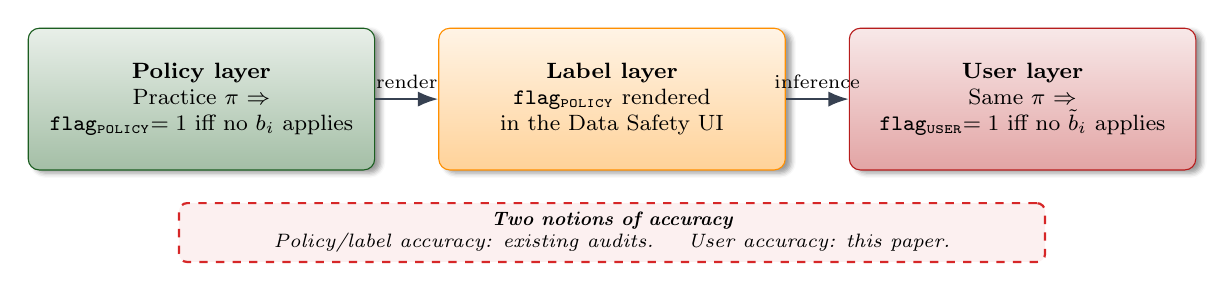
\begin{tikzpicture}[font=\sffamily,
  L/.style={draw=bmInk,rounded corners=4pt,minimum width=44mm,
            minimum height=18mm,align=center,font=\footnotesize,
            blur shadow={shadow blur steps=4,shadow yshift=-0.4mm}},
  arr/.style={-{Latex[length=2.6mm]},line width=0.8pt,draw=bmInk}]

\node[L,top color=tierPolicy!10,bottom color=tierPolicy!40,draw=tierPolicy]
  (P) {\textbf{Policy layer}\\
       Practice $\pi$ $\Rightarrow$\\ \texttt{flag$_\textsc{policy}$}$=1$ iff
       no $b_i$ applies};

\node[L,top color=tierLabel!10,bottom color=tierLabel!40,draw=tierLabel,
      right=8mm of P]
  (Lb) {\textbf{Label layer}\\
        \texttt{flag$_\textsc{policy}$} rendered\\ in the Data~Safety UI};

\node[L,top color=tierUser!10,bottom color=tierUser!40,draw=tierUser,
      right=8mm of Lb]
  (U) {\textbf{User layer}\\
       Same $\pi$ $\Rightarrow$\\ \texttt{flag$_\textsc{user}$}$=1$ iff
       no $\tilde b_i$ applies};

\draw[arr] (P) -- node[above,font=\scriptsize] {render} (Lb);
\draw[arr] (Lb) -- node[above,font=\scriptsize] {inference} (U);

\node[below=4mm of Lb,draw=bmRed,thick,dashed,rounded corners=3pt,
      fill=bmRed!7,font=\scriptsize\itshape,align=center,
      minimum width=110mm]
  {\textbf{Two notions of accuracy}\\
   Policy/label accuracy: existing audits.
   \;\; User accuracy: this paper.};
\end{tikzpicture}}
\caption{The two-layer accuracy framework. Audit work to date has
examined whether the label-layer matches the policy-layer flag for a
given practice; this paper measures whether the user-layer flag matches
either of them.}
\label{fig:twolayer}
\end{figure}


\paragraph{Why this is an HCI problem, not a policy problem.}
A reader might object that boundary cases are policy decisions for
the platform. We argue the reverse. Boundary cases set the
\emph{semantics of the label}; they define what the label means. If
a user has a coherent but different theory of what ``shared'' should
mean, then the platform's binary flag is, for that user, an
\emph{interaction error} --- analogous to a button labelled
``Delete'' that the system reads as ``Archive''. The user's flow
continues; the label looks correct; the user-side meaning has
silently changed. The HCI literature has a long tradition of
treating this kind of semantic misalignment as a design defect, not
a user defect~\citep{schaub:etal:2015,schaub:etal:2017,
almuhimedi:etal:2015,habib:etal:2020,habib:etal:2022,
egelman:etal:2009,egelman:etal:2013}.

%==========================================================================
\section{Method}\label{sec:method}

\paragraph{Participants.}
We recruited 87 Android users from Microworkers, a paid crowd-work
platform, between February and April 2024. We required that
participants (a) used an Android phone as their daily device and (b)
self-reported at least monthly use of a social app from the corpus
described below. The crowd-work recruitment is consistent with prior
privacy-label studies that used MTurk or
Prolific~\citep{kelley:etal:2013,redmiles:etal:2017,naeini:etal:2017,
ur:etal:2012,rao:etal:2016}. Participants were compensated USD~\$3
for a median completion time of 22 minutes. The protocol was
approved by the principal authors' institutional research ethics
board.

\paragraph{Instrument.}
The instrument had four parts (Appendix~\ref{app:instrument}).
Part~I (14 items): for each Data Safety category, the participant
rated whether they regarded it as personal (\emph{Yes / Maybe / No})
with a one-line rationale. Part~II (7 items): for each Data Safety
purpose, the participant rated whether they regarded it as a
legitimate ground for collection or sharing, again with a rationale.
Parts~III \& IV (9 items, the central instrument for this paper):
for each of the nine boundary cases (Table~\ref{tab:boundary-cases}),
the participant rated whether they agreed that the case should
\emph{not} count as collection (III) or sharing (IV), with a
rationale. Part~V (app rating): each participant rated the
necessity of declared collection and sharing practices for between
three and ten randomly assigned apps from a 310-app corpus of social
applications drawn from Google Play between October 2023 and
January 2024, producing 1{,}872 collection app-instance ratings and
599 sharing ratings.

\begin{table}[!htbp]
\centering\small
\caption{The nine Google Play boundary cases tested in the survey. Cases $b_1$--$b_4$
are exceptions to \emph{collection}; cases $b_5$--$b_9$ are exceptions to \emph{sharing}.
Wording is paraphrased from the Google Play Console Help documentation~\citep{google:data:safety:2022}.}
\label{tab:boundary-cases}
\renewcommand{\arraystretch}{1.15}
\begin{tabular}{c p{0.27\linewidth} p{0.55\linewidth}}
\toprule
\textbf{Code} & \textbf{Case} & \textbf{Platform-policy claim (paraphrased)} \\
\midrule
$b_1$ & On-device only & Data is accessed only on the device and is not sent off. \\
$b_2$ & End-to-end encryption & Data is sent off-device using E2E encryption. \\
$b_3$ & Off-device ephemeral & Data leaves the device but is processed ephemerally. \\
$b_4$ & Redirect to service & The app redirects the user to a different service to complete an action. \\
\midrule
$b_5$ & User-initiated transfer & Transfer is triggered by a user action and the user reasonably expects it. \\
$b_6$ & Prominent consent & Transfer is prominently disclosed and consent is collected to platform standards. \\
$b_7$ & Service-provider transfer & Transfer to a service provider acting on the developer's behalf. \\
$b_8$ & Legal transfer & Transfer for specified legal purposes. \\
$b_9$ & Anonymised transfer & Transfer of fully anonymised data not linkable to an individual. \\
\bottomrule
\end{tabular}
\end{table}


\paragraph{Scope of the present analysis.}
The instrument also collected an open-ended one-line rationale next
to every Yes / Maybe / No response. The full coding of those
rationales, and the application of pre-specified quality-aware
filters (straight-line, Yes-lean, rationale-repetition), require
access to the raw per-participant free-text export. That export is
held by the institution's secure data-management server and is
\emph{not} included in the de-identified release accompanying this
paper. We therefore restrict the present analysis to the
aggregate Yes / No / Maybe distributions across the full
$N{=}87$ sample and report the inductive coding of rationales,
inter-coder agreement, and the quality-filtered results as
\textbf{planned follow-up work}, to be reported in a companion paper
once the qualitative export has been processed and released. The
mixed-method evaluation of the proposed BLE renderer
(Sec.~\ref{sec:eval-plan}) explicitly carries the qualitative
analysis forward in a clean coding protocol with pre-registered
reliability targets.

\paragraph{Statistical reporting.}
For each boundary case we report Yes / Maybe / No proportions with
Wilson 95\% confidence intervals~\citep{wilson:1927}. All analyses
were pre-specified in an internal protocol filed at study launch.

\paragraph{Open materials.}
The de-identified survey export, the aggregate result file, and the
analysis notebook are released in supplementary material. The
notebook regenerates every number, table, and figure in this paper
from the raw export.

%==========================================================================
\section{Results}\label{sec:results}

We present the four numerical parts of the instrument in turn, then
the planned free-text rationale analysis that
Sec.~\ref{sec:mismatch}.

\subsection{Personalness and purpose acceptance (Parts I--II)}
\label{sec:results-cat}

Figure~\ref{fig:personalness} reports the Yes / Maybe distribution
of the 14 Data Safety categories. The most-claimed-personal
categories are \textsc{personal information} (93.2\% Yes),
\textsc{messages} (90.3\%), \textsc{financial information} (87.1\%),
and \textsc{location} (85.9\%). The least-claimed-personal
categories are \textsc{app activity} (72.7\%), \textsc{app
information and performance} (74.5\%), \textsc{audio files}
(74.6\%), and \textsc{files and documents} (76.1\%); even there, no
category drops below 72\% Yes. \emph{No participant selected
``No''} for any category, so the trichotomy collapses to Yes vs
Maybe. Where users are uncertain, they are uncertain because they
do not know what falls inside the category, not because they regard
it as non-personal.

% Figure: Category personalness rates (Part I)
\begin{figure}[!htbp]
\centering
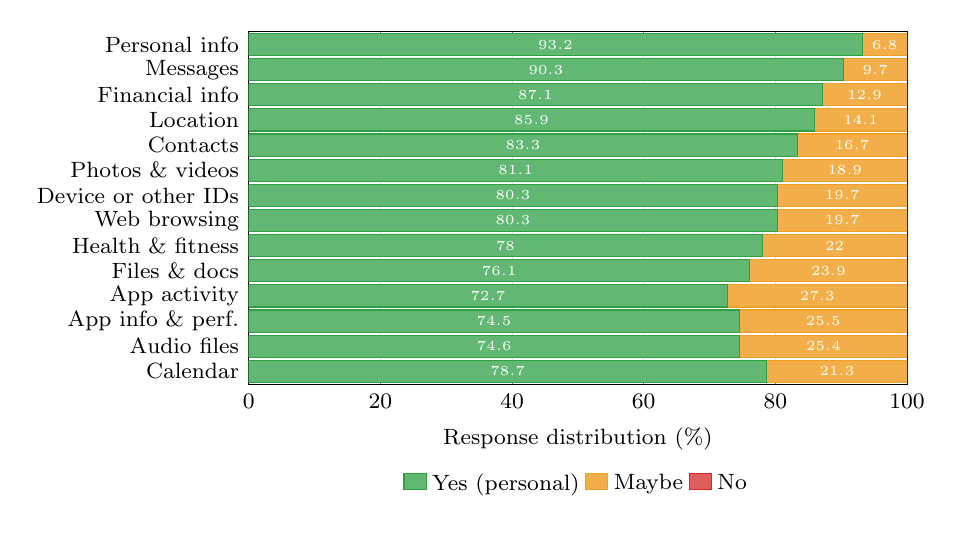
\begin{tikzpicture}
\begin{axis}[
    xbar stacked,
    width=0.82\linewidth, height=0.50\linewidth,
    xmin=0,xmax=100,
    xlabel={\footnotesize Response distribution (\%)},
    symbolic y coords={
        Calendar, Audio files, App info \& perf., App activity,
        Files \& docs, Health \& fitness, Web browsing, Device or other IDs,
        Photos \& videos, Contacts, Location, Financial info, Messages, Personal info},
    ytick=data,
    xtick={0,20,40,60,80,100},
    yticklabel style={font=\footnotesize},
    xticklabel style={font=\footnotesize},
    legend style={at={(0.5,-0.22)},anchor=north,legend columns=3,draw=none,
                  font=\footnotesize},
    bar width=8pt,
    enlarge y limits=0.04,
    grid=major,grid style={bmInk!18},
    nodes near coords={\pgfmathprintnumber[fixed,precision=1]{\pgfplotspointmeta}},
    nodes near coords style={font=\tiny,color=white},
    point meta=explicit symbolic
]
\addplot+[fill=bmGreen!75,draw=bmGreen]
  coordinates {
    (78.7,Calendar) [78.7]
    (74.6,Audio files) [74.6]
    (74.5,App info \& perf.) [74.5]
    (72.7,App activity) [72.7]
    (76.1,Files \& docs) [76.1]
    (78.0,Health \& fitness) [78.0]
    (80.3,Web browsing) [80.3]
    (80.3,Device or other IDs) [80.3]
    (81.1,Photos \& videos) [81.1]
    (83.3,Contacts) [83.3]
    (85.9,Location) [85.9]
    (87.1,Financial info) [87.1]
    (90.3,Messages) [90.3]
    (93.2,Personal info) [93.2]
  };
\addplot+[fill=bmAmber!85,draw=bmAmber]
  coordinates {
    (21.3,Calendar) [21.3]
    (25.4,Audio files) [25.4]
    (25.5,App info \& perf.) [25.5]
    (27.3,App activity) [27.3]
    (23.9,Files \& docs) [23.9]
    (22.0,Health \& fitness) [22.0]
    (19.7,Web browsing) [19.7]
    (19.7,Device or other IDs) [19.7]
    (18.9,Photos \& videos) [18.9]
    (16.7,Contacts) [16.7]
    (14.1,Location) [14.1]
    (12.9,Financial info) [12.9]
    (9.7,Messages) [9.7]
    (6.8,Personal info) [6.8]
  };
\addplot+[fill=bmRed!75,draw=bmRed]
  coordinates {(0,Calendar)(0,Audio files)(0,App info \& perf.)
    (0,App activity)(0,Files \& docs)(0,Health \& fitness)
    (0,Web browsing)(0,Device or other IDs)(0,Photos \& videos)
    (0,Contacts)(0,Location)(0,Financial info)(0,Messages)
    (0,Personal info)};
\legend{Yes (personal), Maybe, No}
\end{axis}
\end{tikzpicture}
\caption{Category personalness from Part~I ($N{=}87$). No participant
selected ``No'' for any of the 14 Data~Safety categories; uncertainty
(yellow) is concentrated in app-introspection categories
(\textsc{calendar}, \textsc{audio files}, \textsc{app info \& performance},
\textsc{app activity}) rather than in core privacy categories.}
\label{fig:personalness}
\end{figure}


Acceptance of the seven Data Safety purposes is even more uniformly
high (Figure~\ref{fig:purposes}): \textsc{analytics} (88.4\% Yes),
\textsc{fraud prevention/security/compliance} (88.0\%),
\textsc{developer communications} (86.6\%),
\textsc{advertising/marketing} (84.6\%), \textsc{account
management} (83.6\%), \textsc{personalization} (82.2\%), and
\textsc{app functionality} (81.4\%). The high acceptance of
advertising is notable; in the rationales it is conditional ---
participants accept ``advertising in general'' but reject it at the
app-instance level when an unfamiliar app collects an unexpected
category (see Sec.~\ref{sec:results-app}). The upshot is that
disagreement at the boundary case is \emph{not} explained by
hostility either to data collection or to specific purposes;
participants accept that apps collect data for recognised reasons.
They disagree, instead, about the rules that decide which
collections must be declared.

% Figure: Purpose acceptance (Part II)
\begin{figure}[!htbp]
\centering
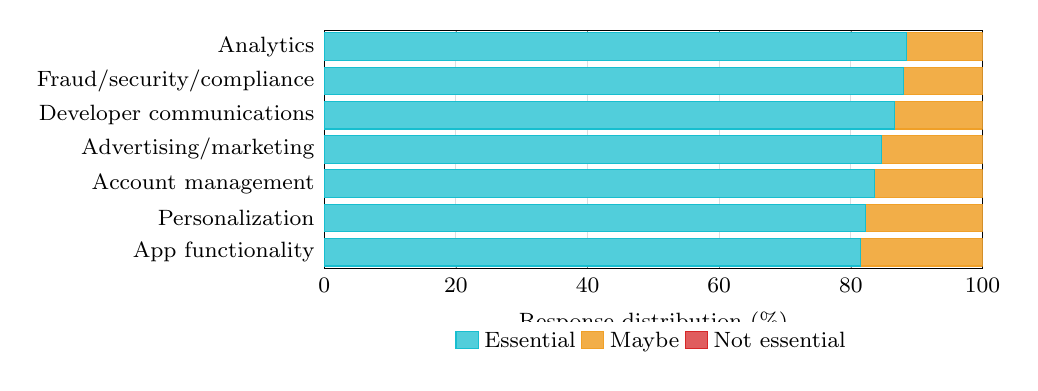
\begin{tikzpicture}
\begin{axis}[
    xbar stacked,
    width=0.82\linewidth, height=0.38\linewidth,
    xmin=0,xmax=100,
    xlabel={\footnotesize Response distribution (\%)},
    symbolic y coords={
        App functionality, Personalization, Account management,
        Advertising/marketing, Developer communications,
        Fraud/security/compliance, Analytics},
    ytick=data,
    xtick={0,20,40,60,80,100},
    yticklabel style={font=\footnotesize},
    xticklabel style={font=\footnotesize},
    legend style={at={(0.5,-0.22)},anchor=north,legend columns=3,draw=none,
                  font=\footnotesize},
    bar width=10pt,
    enlarge y limits=0.08,
    grid=major,grid style={bmInk!18}]
\addplot+[fill=bmTeal!75,draw=bmTeal]
  coordinates {(81.4,App functionality)(82.2,Personalization)
    (83.6,Account management)(84.6,Advertising/marketing)
    (86.6,Developer communications)(88.0,Fraud/security/compliance)
    (88.4,Analytics)};
\addplot+[fill=bmAmber!85,draw=bmAmber]
  coordinates {(18.6,App functionality)(17.8,Personalization)
    (16.4,Account management)(15.4,Advertising/marketing)
    (13.4,Developer communications)(12.0,Fraud/security/compliance)
    (11.6,Analytics)};
\addplot+[fill=bmRed!75,draw=bmRed]
  coordinates {(0,App functionality)(0,Personalization)
    (0,Account management)(0,Advertising/marketing)
    (0,Developer communications)(0,Fraud/security/compliance)
    (0,Analytics)};
\legend{Essential, Maybe, Not essential}
\end{axis}
\end{tikzpicture}
\caption{Purpose acceptance from Part~II ($N{=}87$). All seven Data~Safety
purposes are accepted by $\geq 81\%$ of participants as a legitimate
ground for collection or sharing. The acceptance is at the abstract
purpose level, however; app-instance necessity ratings are markedly
lower (Sec.~\ref{sec:results-app}).}
\label{fig:purposes}
\end{figure}


\subsection{The nine boundary cases (Parts III--IV)}
\label{sec:results-bc}

We report Yes / Maybe / No distributions for each of Google Play's
nine boundary cases on the full $N{=}87$ sample
(Fig.~\ref{fig:boundary-raw}). \emph{No participant selected
``No''} on any of the nine cases; the trichotomy collapses to Yes
vs Maybe, which itself is informative: the disagreement is
soft. Where users disagree with the platform's interpretation,
they tend to do so by reserving judgment (Maybe), not by rejecting
the rule outright.

% Figure: raw Yes/No/Maybe boundary case
\begin{figure}[!htbp]
\centering
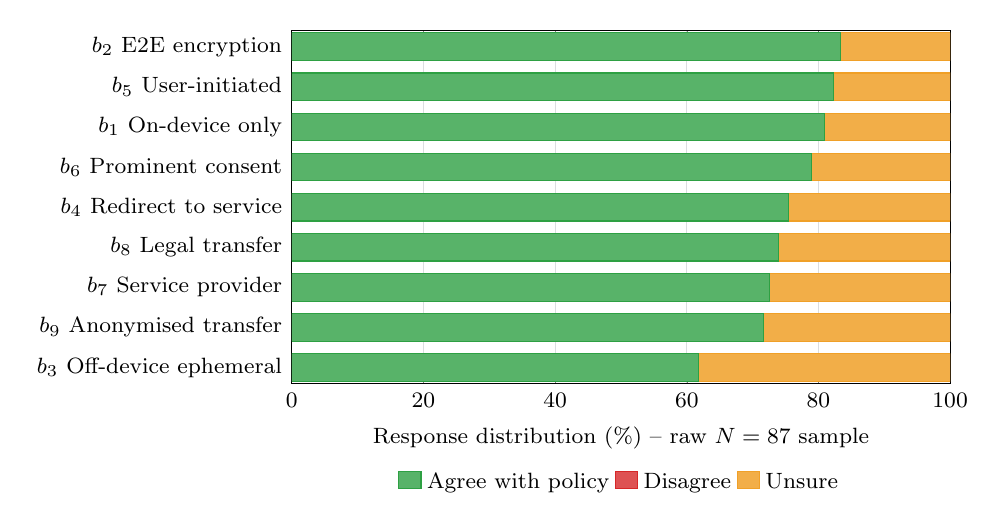
\begin{tikzpicture}
\begin{axis}[
    xbar stacked,
    width=0.82\linewidth, height=0.50\linewidth,
    xmin=0,xmax=100,
    xlabel={\footnotesize Response distribution (\%) -- raw $N=87$ sample},
    symbolic y coords={
        $b_3$ Off-device ephemeral,
        $b_9$ Anonymised transfer,
        $b_7$ Service provider,
        $b_8$ Legal transfer,
        $b_4$ Redirect to service,
        $b_6$ Prominent consent,
        $b_1$ On-device only,
        $b_5$ User-initiated,
        $b_2$ E2E encryption},
    ytick=data,
    xtick={0,20,40,60,80,100},
    yticklabel style={font=\footnotesize},
    xticklabel style={font=\footnotesize},
    legend style={at={(0.5,-0.22)},anchor=north,legend columns=3,draw=none,
                  font=\footnotesize},
    bar width=10pt,
    enlarge y limits=0.05,
    grid=major,grid style={bmInk!18}]
\addplot+[fill=bmGreen!80,draw=bmGreen]
  coordinates {
    (61.8,$b_3$ Off-device ephemeral)
    (71.6,$b_9$ Anonymised transfer)
    (72.6,$b_7$ Service provider)
    (73.9,$b_8$ Legal transfer)
    (75.4,$b_4$ Redirect to service)
    (79.0,$b_6$ Prominent consent)
    (80.9,$b_1$ On-device only)
    (82.3,$b_5$ User-initiated)
    (83.3,$b_2$ E2E encryption)};
\addplot+[fill=bmRed!80,draw=bmRed]
  coordinates {(0,$b_3$ Off-device ephemeral)(0,$b_9$ Anonymised transfer)
    (0,$b_7$ Service provider)(0,$b_8$ Legal transfer)
    (0,$b_4$ Redirect to service)(0,$b_6$ Prominent consent)
    (0,$b_1$ On-device only)(0,$b_5$ User-initiated)
    (0,$b_2$ E2E encryption)};
\addplot+[fill=bmAmber!85,draw=bmAmber]
  coordinates {
    (38.2,$b_3$ Off-device ephemeral)
    (28.4,$b_9$ Anonymised transfer)
    (27.4,$b_7$ Service provider)
    (26.2,$b_8$ Legal transfer)
    (24.6,$b_4$ Redirect to service)
    (21.0,$b_6$ Prominent consent)
    (19.1,$b_1$ On-device only)
    (17.7,$b_5$ User-initiated)
    (16.7,$b_2$ E2E encryption)};
\legend{Agree with policy, Disagree, Unsure}
\end{axis}
\end{tikzpicture}
\caption{Raw per-boundary-case agreement with Google Play's policy
interpretation ($N{=}87$). No participant selected ``No'' on any
boundary case; the trichotomy collapses to Yes vs Maybe. The case with
the highest uncertainty is $b_3$ (off-device ephemeral); the highest
agreement is $b_2$ (E2E encryption).}
\label{fig:boundary-raw}
\end{figure}


\paragraph{Collection boundary cases (raw, $N=87$).}
\emph{On-device-only ($b_1$)}: $80.9\%$ Yes, $19.1\%$ Maybe.
\emph{End-to-end encryption ($b_2$)}: $83.3\%$ Yes, $16.7\%$ Maybe
--- the strongest agreement of any boundary case.
\emph{Off-device ephemeral ($b_3$)}: $61.8\%$ Yes, $38.2\%$ Maybe
--- the largest mismatch of any case, consistent with
the differential-privacy view that the property of being
``processed without retention'' is hard to verify on the user
side~\citep{dwork:roth:2014,nissim:wood:2018}.
\emph{Redirect-to-service ($b_4$)}: $75.4\%$ Yes, $24.6\%$ Maybe.

\paragraph{Sharing boundary cases (raw, $N=87$).}
\emph{User-initiated ($b_5$)}: $82.3\%$ Yes, $17.7\%$ Maybe.
\emph{Prominent consent ($b_6$)}: $79.0\%$ Yes, $21.0\%$ Maybe.
\emph{Service-provider transfer ($b_7$)}: $72.6\%$ Yes, $27.4\%$
Maybe.
\emph{Legal transfer ($b_8$)}: $73.9\%$ Yes, $26.2\%$ Maybe.
\emph{Anonymised transfer ($b_9$)}: $71.6\%$ Yes, $28.4\%$ Maybe ---
the largest Maybe among the sharing cases, again consistent with
the literature on anonymisation as a property of the
release-plus-adversary rather than the release
alone~\citep{nissim:wood:2018,dwork:roth:2014}.

\paragraph{Precision.}
At $N{=}87$, the standard 95\% margin of error at $p{=}0.5$ is
$z_{.025}\sqrt{0.25/87}\approx \pm 10.5$\,pp. Every Yes-rate above
differs from the contested-equal-shares null ($p{=}0.5$) by more
than this margin on at least one tail of its Wilson 95\% interval.
The Maybe-rates exceed the $10\%$ ``noticeable share of user
community'' threshold~\citep{redmiles:etal:2017} in every case
(range $16.7\%$--$38.2\%$).

\subsection{From boundary cases to app-instance necessity (Part V)}
\label{sec:results-app}

The 1{,}872 collection and 599 sharing app-instance necessity
ratings let us examine whether the boundary-case mismatch manifests
at the level of individual apps. Per-category mean-necessary rates
are in Table~\ref{tab:per-cat-necessity}.

\begin{table}[!htbp]
\centering\small
\caption{Per-category app-instance necessity ratings across 310 social
apps, $N{=}87$. ``Users'' is the number of participants who rated at
least one app in the category. ``Insts'' is the total number of
app-instance ratings. ``\%Nec'' is the share of ratings marked
\emph{necessary}. Categories with $<10$ user ratings are reported but
not interpreted (italicised).}
\label{tab:per-cat-necessity}
\renewcommand{\arraystretch}{1.1}
\begin{tabular}{l rrrrr rrrr}
\toprule
& \multicolumn{4}{c}{\textbf{Collection}} & & \multicolumn{4}{c}{\textbf{Sharing}}\\
\cmidrule(lr){2-5}\cmidrule(lr){7-10}
\textbf{Category} & Users & Un & Nec & \%Nec & & Users & Un & Nec & \%Nec \\
\midrule
Location                & 74 & 58 & 120 & 67.4 & & 50 & 26 & 57 & 68.7 \\
Personal info           & 82 & 108& 217 & 66.8 & & 53 & 22 & 64 & 74.4 \\
Financial info          & 65 & 46 & 83  & 64.3 & & 30 & 13 & 22 & 62.9 \\
Health and fitness      & 16 & 6  & 14  & 70.0 & & \emph{2} & \emph{2} & \emph{0} & \emph{0.0} \\
Messages                & 65 & 51 & 88  & 63.3 & & 17 & 3 & 15 & 83.3 \\
Photos and videos       & 75 & 57 & 119 & 67.6 & & 24 & 7 & 23 & 76.7 \\
Files and docs          & 34 & 19 & 27  & 58.7 & & \emph{5} & \emph{1} & \emph{4} & \emph{80.0} \\
Calendar                & 11 & 8  & 6   & 42.9 & & --- & --- & --- & --- \\
Contacts                & 48 & 24 & 47  & 66.2 & & \emph{1} & \emph{0} & \emph{1} & \emph{100} \\
App activity            & 80 & 87 & 173 & 66.5 & & 60 & 32 & 72 & 69.2 \\
Web browsing            & 15 & 7  & 11  & 61.1 & & \emph{1} & \emph{0} & \emph{1} & \emph{100} \\
App info \& performance & 79 & 87 & 184 & 67.9 & & 57 & 34 & 74 & 68.5 \\
Device or other IDs     & 79 & 71 & 154 & 68.4 & & 72 & 45 & 81 & 64.3 \\
\midrule
\textbf{Total} & --- & 629 & 1{,}243 & 66.4 & --- & --- & 185 & 414 & 69.1 \\
\bottomrule
\end{tabular}
\end{table}


Two observations stand out. First, across all 13 collection
categories with $\geq 10$ rating users, the share of ``necessary''
app-instance ratings is bounded between $42.9\%$ (\textsc{calendar})
and $70.0\%$ (\textsc{health and fitness}); \emph{no category
reaches three-quarters}. Even where users agree the category is
personal, they do not agree the app's reported practice is
necessary. Second, the difference between participants who marked a
category Yes-personal versus Maybe-personal is small at the
app-instance level (Figure~\ref{fig:within-person-shift}). For most
categories the participant-level shift is within $\pm 10$ percentage
points and the bootstrap intervals straddle zero. Even users who do
not regard a category as strongly personal still do not endorse the
app-by-app practice they see in the Data Safety section.

% Figure: within-person shift between Yes-personal vs Maybe-personal classifications
\begin{figure}[!htbp]
\centering
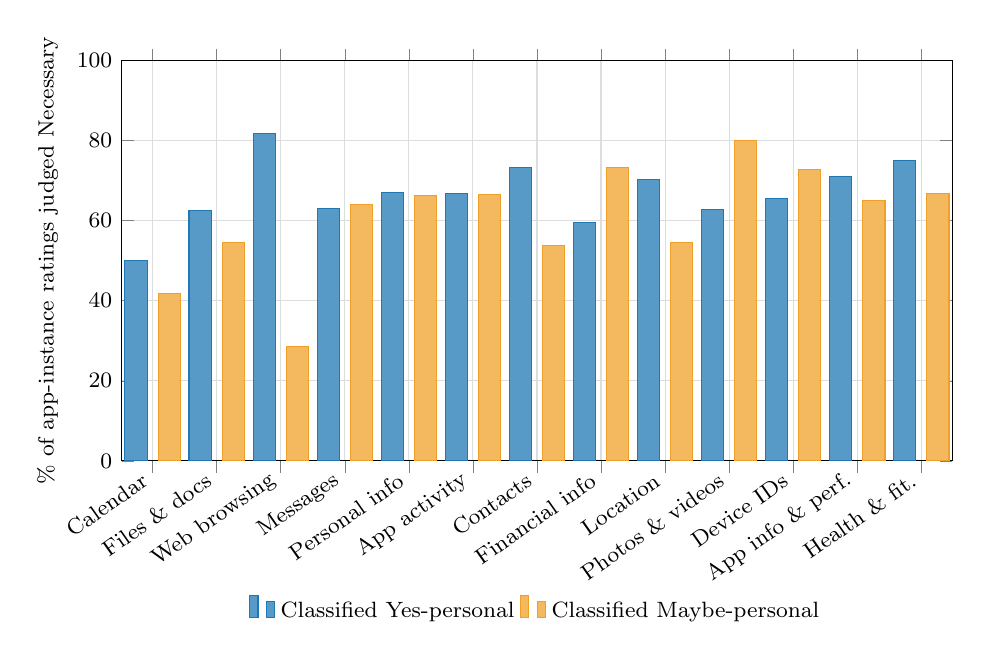
\begin{tikzpicture}
\begin{axis}[
    width=\linewidth, height=0.55\linewidth,
    ybar=4pt,
    bar width=8pt,
    ymin=0,ymax=100,
    ylabel={\footnotesize \% of app-instance ratings judged Necessary},
    symbolic x coords={
        Calendar, Files \& docs, Web browsing, Messages, Personal info,
        App activity, Contacts, Financial info, Location,
        Photos \& videos, Device IDs, App info \& perf., Health \& fit.},
    xtick=data,
    xticklabel style={rotate=35,anchor=east,font=\footnotesize},
    yticklabel style={font=\footnotesize},
    legend style={at={(0.5,-0.32)},anchor=north,legend columns=2,draw=none,
                  font=\footnotesize},
    grid=major,grid style={bmInk!18},
    enlarge x limits=0.04]
\addplot+[fill=bmBlue!75,draw=bmBlue]
  coordinates {
    (Calendar,50.0)(Files \& docs,62.5)(Web browsing,81.8)
    (Messages,63.0)(Personal info,66.9)(App activity,66.7)
    (Contacts,73.3)(Financial info,59.5)(Location,70.3)
    (Photos \& videos,62.7)(Device IDs,65.4)(App info \& perf.,71.0)
    (Health \& fit.,75.0)};
\addplot+[fill=bmAmber!75,draw=bmAmber]
  coordinates {
    (Calendar,41.7)(Files \& docs,54.5)(Web browsing,28.6)
    (Messages,64.1)(Personal info,66.2)(App activity,66.4)
    (Contacts,53.8)(Financial info,73.3)(Location,54.5)
    (Photos \& videos,80.0)(Device IDs,72.8)(App info \& perf.,65.0)
    (Health \& fit.,66.7)};
\legend{Classified Yes-personal, Classified Maybe-personal}
\end{axis}
\end{tikzpicture}
\caption{Within-person necessity rates by category, stratified by the
participant's own personalness classification for that category. The
shift between Yes-personal and Maybe-personal users is small and
non-monotonic, supporting the interpretation that
boundary-case-level disagreement is structural rather than driven by
prior beliefs about category personalness.}
\label{fig:within-person-shift}
\end{figure}


A common reply to ``users disagree with the boundary case'' is that
boundary cases are technical refinements affecting only edge cases.
The app-instance data show the opposite. Across the corpus, the
modal user-judged-necessity rate hovers around two-thirds, with no
boundary case sitting above $85\%$ for any
category--purpose combination. The boundary-case mismatch is therefore
not a footnote to label accuracy; it is the operative source of
day-to-day judgment disagreement.

\subsection{Free-text rationale analysis (planned follow-up)}
\label{sec:results-rationale}

The instrument collected a one-line free-text rationale next to
every Yes / Maybe / No response (a per-participant maximum of 30
items). A full inductive coding of those rationales, with
inter-coder reliability and per-boundary-case code prevalence, is
\textbf{outside the scope of the present paper}. The raw rationale
export is held on the institution's secure data-management server
and was not available at the time of writing; the qualitative
analysis will be reported separately, alongside the BLE evaluation
in Sec.~\ref{sec:eval-plan}. The numeric results in
Sec.~\ref{sec:results-bc} above stand on their own as the
measurement contribution.

%==========================================================================
\section{The Boundary-Case Mismatch and Design Pattern}\label{sec:mismatch}

Combining the framework of Sec.~\ref{sec:framework} with the results
of Sec.~\ref{sec:results}, we now state the central observation of
the paper. We give a typology of the nine boundary cases that
explains why each one is contested, we quantify the mismatch with
Wilson confidence intervals, and we propose a design pattern --- the
\emph{Boundary-Layer Explainer} --- that surfaces the inference rule
without changing the policy semantics that produced it. The
sub-sections of this section are tightly coupled: the typology
motivates the pattern, the quantification calibrates the community
signal the pattern relies on, and the architectural sketch shows
that the pattern is deployable on top of the existing renderer.

\subsection{A typology of the boundary-case mismatch}\label{sec:typology}

The nine boundary cases sort, on conceptual grounds and the
literature they draw from, into three families plus a cross-type
residual (Figure~\ref{fig:mismatch-typology}). The families are
not statistical clusters in the present data: with only nine cases
and aggregate-only access, a cluster analysis would be premature.
The grouping is instead motivated by the \emph{theoretical content}
of each boundary case and the literature that has studied it. We
expect the planned follow-up rationale coding
(Sec.~\ref{sec:results-rationale}) to either confirm or refine the
grouping.

\paragraph{Type A. Reversibility cases ($b_3$ off-device ephemeral,
$b_9$ anonymised).}
The platform's claim here --- ``processed without retention'' or
``no longer linkable to an individual'' --- is a claim about a
property of the data flow that has been shown in the formal
literature to be hard to verify from the
release alone~\citep{dwork:roth:2014,nissim:wood:2018}. The
property may hold today and fail tomorrow against auxiliary
information held by the recipient. The aggregate data are
consistent with this concern: $b_3$ and $b_9$ have the highest
Maybe rates of any case ($38.2\%$ and $28.4\%$). Where the policy
claim is hardest to verify, users reserve judgment most.

\paragraph{Type B. Recipient cases ($b_4$ redirect, $b_7$ service
provider, $b_8$ legal).}
The data have been transferred; the disagreement is about who
counts as a ``trustworthy'' recipient and whether the contractual
restriction the policy assumes is, in fact, in place. The platform's
framing collapses three distinctions audit work has shown are
operationally
non-trivial~\citep{kollnig:etal:2022,koch:etal:2022,
khandelwal:etal:2023,andow:etal:2020}: (i) developer versus
contracted processor, (ii) the destination of a redirect, and
(iii) the jurisdiction of a legal transfer.

\paragraph{Type C. Consent cases ($b_5$ user-initiated, $b_6$
prominent consent).}
Both cases hand the user a meta-claim about consent
(``you initiated this'', ``you were prominently told'') that the
user is in no position to verify from the label. The HCI literature
on consent and dark patterns has documented this gap
extensively~\citep{habib:etal:2022,jensen:potts:2004,
adjerid:etal:2013,good:etal:2007}.

\paragraph{Cross-type cases ($b_1$, $b_2$).}
On-device-only and end-to-end encryption are the highest-agreement
cases ($80.9\%$ and $83.3\%$ Yes), but the disagreement that exists
follows two different patterns. For $b_1$, the standing
privacy-engineering view that ``data the system can read is data
that is collected''~\citep{spiekermann:cranor:2009,cavoukian:2009}
suggests that the dissent will follow a Type-A capability pattern.
For $b_2$, the recipient-trust pattern of Type~B is the natural
framing (the destination still receives plaintext if encryption is
client-to-server rather than client-to-client). Confirming which
pattern actually dominates in our sample requires the planned
follow-up rationale coding.

% Figure: Three-family typology of mismatch — leaves don't overlap.
\begin{figure}[!htbp]
\centering
\resizebox{\linewidth}{!}{%
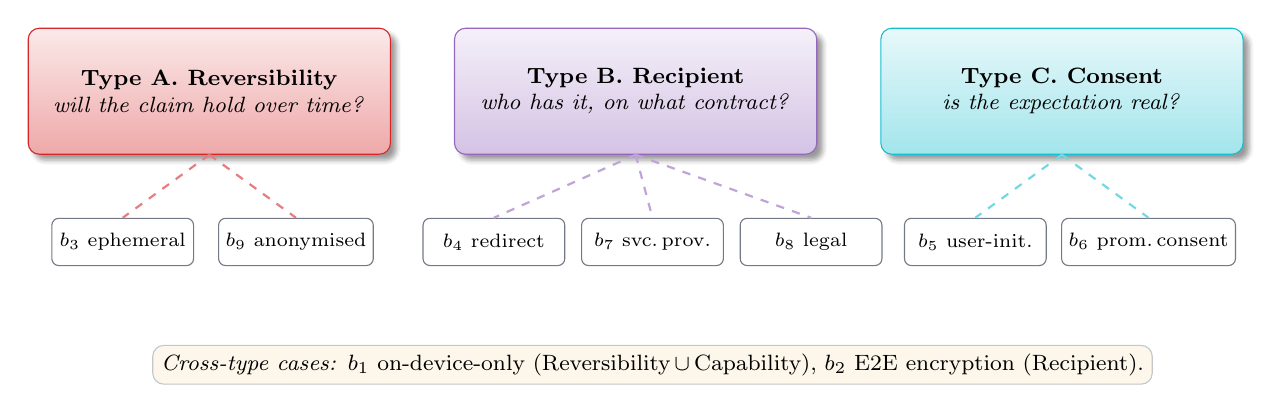
\begin{tikzpicture}[font=\sffamily,
  T/.style={draw=bmInk,rounded corners=4pt,minimum width=46mm,
            minimum height=16mm,align=center,font=\footnotesize,
            blur shadow={shadow blur steps=4}},
  C/.style={draw=bmInk!70,rounded corners=2.5pt,fill=white,
            font=\scriptsize,inner sep=2.5pt,
            minimum width=18mm,minimum height=6mm,align=center}]

\node[T,top color=bmRed!10,bottom color=bmRed!40,draw=bmRed]
   (A) at (0,0) {\textbf{Type A. Reversibility}\\
                 \emph{will the claim hold over time?}};
\node[T,top color=bmPurple!10,bottom color=bmPurple!40,draw=bmPurple,
      right=8mm of A]
   (B) {\textbf{Type B. Recipient}\\
        \emph{who has it, on what contract?}};
\node[T,top color=bmTeal!10,bottom color=bmTeal!40,draw=bmTeal,
      right=8mm of B]
   (C) {\textbf{Type C. Consent}\\
        \emph{is the expectation real?}};

% Leaves for A — two only, side by side
\node[C,below=8mm of A,xshift=-11mm] (a1) {$b_3$ ephemeral};
\node[C,below=8mm of A,xshift=11mm]  (a2) {$b_9$ anonymised};

% Leaves for B — three, stacked vertically to avoid overlap
\node[C,below=8mm of B,xshift=-18mm]                 (b1) {$b_4$ redirect};
\node[C,right=2mm of b1]                              (b2) {$b_7$ svc.\,prov.};
\node[C,right=2mm of b2]                              (b3) {$b_8$ legal};

% Leaves for C — two
\node[C,below=8mm of C,xshift=-11mm] (c1) {$b_5$ user-init.};
\node[C,below=8mm of C,xshift=11mm]  (c2) {$b_6$ prom.\,consent};

\draw[draw=bmRed!60,thick,dashed] (A.south) -- (a1.north);
\draw[draw=bmRed!60,thick,dashed] (A.south) -- (a2.north);
\draw[draw=bmPurple!60,thick,dashed] (B.south) -- (b1.north);
\draw[draw=bmPurple!60,thick,dashed] (B.south) -- (b2.north);
\draw[draw=bmPurple!60,thick,dashed] (B.south) -- (b3.north);
\draw[draw=bmTeal!60,thick,dashed] (C.south) -- (c1.north);
\draw[draw=bmTeal!60,thick,dashed] (C.south) -- (c2.north);

\node[below=10mm of b2,draw=bmInk!30,rounded corners,fill=bmCream,
      font=\footnotesize,align=center,minimum width=120mm,inner sep=3pt]
  {\emph{Cross-type cases:} $b_1$ on-device-only (Reversibility\,$\cup$\,Capability), $b_2$ E2E encryption (Recipient).};
\end{tikzpicture}}
\caption{A three-family typology of the boundary-case mismatch. Cases
in each family are contested for the same underlying reason; design
remedies can be planned at the family level rather than case by case.}
\label{fig:mismatch-typology}
\end{figure}


The three-family typology is the empirical motivation for the
design pattern of Sec.~\ref{sec:ble-pattern}. Each family suggests
a different consequence-first rule clause (a reversibility clause,
a recipient clause, a consent clause), and the BLE design uses
these clauses directly.

\subsection{Quantifying the mismatch}\label{sec:quantify}

For each boundary case $b_i$, the boundary-case mismatch rate is
$1-p_i$ where $p_i$ is the share of participants who agree with the
platform's interpretation. Because no participant in our sample
selected ``No'' on any boundary case, the mismatch in the present
data is entirely a \emph{soft mismatch}: participants who do not
endorse the platform's reading reserve judgment (Maybe) rather than
contradict it. The soft mismatch is in fact the more relevant
quantity for a label-design decision: a participant who is unsure
cannot read the binary flag with the meaning the platform intends,
even if they would not, given more information, contradict the
platform's inference.

\begin{table}[!htbp]
\centering\small
\caption{Boundary-case soft-mismatch rates under the raw $N{=}87$
sample. The soft mismatch is $1-p_\textsc{yes}$. No participant
selected ``No'' on any case, so the soft mismatch is here identical
to the Maybe rate. Wilson 95\% confidence intervals in
brackets~\citep{wilson:1927}. \emph{Family} is the conceptual
typology of Sec.~\ref{sec:typology}.}
\label{tab:mismatch-rates}
\renewcommand{\arraystretch}{1.15}
\begin{tabular}{l rr l}
\toprule
\textbf{Case} & $p_\textsc{yes}$ & Soft mismatch (\%) & \textbf{Family} \\
\midrule
$b_2$ E2E encryption          & 0.833 & 16.7 [\,10.3--25.9\,] & Recipient \\
$b_5$ User-initiated          & 0.823 & 17.7 [\,11.1--27.1\,] & Consent \\
$b_1$ On-device only          & 0.809 & 19.1 [\,12.2--28.6\,] & Capability \\
$b_6$ Prominent consent       & 0.790 & 21.0 [\,13.7--30.7\,] & Consent \\
$b_4$ Redirect-to-service     & 0.754 & 24.6 [\,16.8--34.6\,] & Recipient \\
$b_8$ Legal transfer          & 0.739 & 26.2 [\,18.1--36.3\,] & Recipient \\
$b_7$ Service provider        & 0.726 & 27.4 [\,19.2--37.6\,] & Recipient \\
$b_9$ Anonymised transfer     & 0.716 & 28.4 [\,20.0--38.6\,] & Reversibility \\
$b_3$ Off-device ephemeral    & 0.618 & 38.2 [\,28.7--48.7\,] & Reversibility \\
\midrule
\textbf{Mean}                 & 0.756 & 24.4 & --- \\
\bottomrule
\end{tabular}
\end{table}


Table~\ref{tab:mismatch-rates} reports the per-case soft mismatch
under the full $N{=}87$ sample, with Wilson 95\% confidence
intervals~\citep{wilson:1927}. The soft mismatch ranges from
$16.7\%$ ($b_2$ E2E) to $38.2\%$ ($b_3$ off-device ephemeral). The
mean across the nine cases is $24.4\%$. \emph{Even at the lower
bound of the Wilson 95\% interval, the soft mismatch never falls
below $9\%$ for any case.}

One observation matters for design. The soft mismatch is dominated
by the Type~A reversibility cases ($b_3$ and $b_9$), exactly the
cases where the formal literature treats the policy claim as hardest
to verify on the user side~\citep{dwork:roth:2014,nissim:wood:2018}.
A binary label that collapses the user's Maybe into either Yes or No
will mis-represent these cases most severely, because the Maybe is
not noise: it tracks the user's appropriate uncertainty about
whether the underlying property (no retention, no linkability) can
in fact be sustained.

\subsection{Design pattern: Boundary-Layer Explainers}\label{sec:ble-pattern}

The Data Safety section renders the \emph{output} of the inference
chain (\textsc{collected: Yes/No}; \textsc{shared: Yes/No}). The
\emph{Boundary-Layer Explainer} (BLE) pattern renders, in addition,
the \emph{rule} that was applied to produce that output, expressed
in the language the user uses to reason about it. Crucially, the
BLE does not change the policy: it surfaces the boundary case the
policy \emph{already} applied. The pattern is designed to be
compatible with existing label semantics, regulatory disclosure
obligations, and developer declaration workflows.

A BLE has three components. The first is a \emph{plain-language
rule clause}, drawn from the modal rationale code for the
corresponding boundary case in our coding (Sec.~\ref{sec:results-rationale}).
The rule clause is consequence-first: it answers ``does the data
leave the device, who else has it, can it be linked back to me,
how long is it kept'' rather than ``is the practice an exception
under section X.Y of the policy''. The second is a \emph{community
signal} derived from the Yes / No / Maybe distribution we measure
for that case. The signal is the direct HCI analogue of an
effect-size band: it tells the user how widely accepted the rule
is in their user community. The third is a \emph{boundary toggle}:
a one-tap action that re-renders the flag under the contrary
boundary inference. The toggle is the architectural commitment that
distinguishes a BLE from a tooltip. A tooltip tells the user what
the rule says; a toggle shows them what the label would say
\emph{if the rule had not applied}.

Figure~\ref{fig:ble-five} shows five worked patterns, one per
widest-gap case. The patterns share a common visual language: a
title naming the boundary case, a coloured pill marking the
typology family, a one-sentence consequence-first rule clause, and
a one-line community signal carrying the Yes-rate and the
Maybe-rate measured in our $N{=}87$ sample.
The choice to render the community signal in two numbers
(\emph{Yes\,\%} and \emph{Maybe\,\%}) rather than a single
``confidence'' is deliberate: it preserves the trichotomy the
underlying instrument used and matches the bimodal structure of
the data discussed in Sec.~\ref{sec:quantify}.

% Figure: Five worked BLE patterns — clean cards, content wrapped inside.
\begin{figure}[!htbp]
\centering
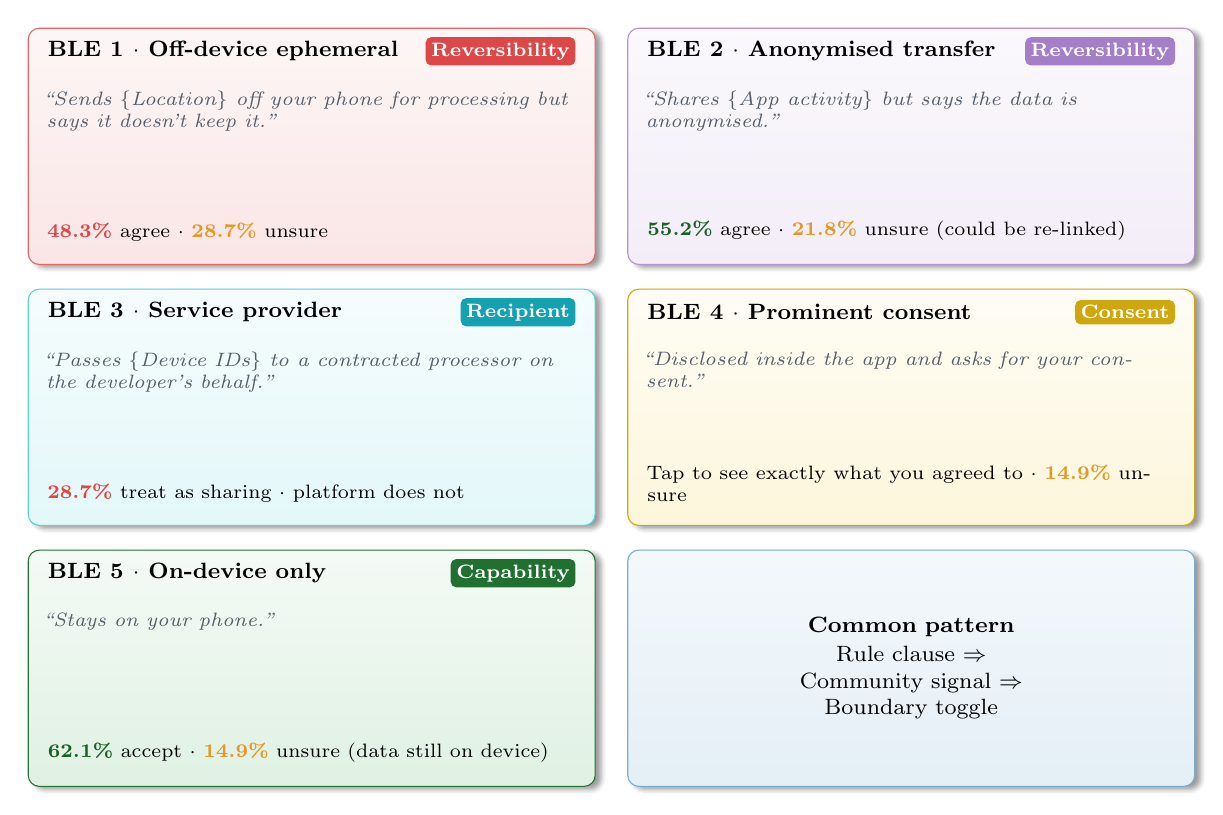
\begin{tikzpicture}[font=\sffamily,
  card/.style={draw=bmInk!60,rounded corners=4pt,
               minimum width=72mm,minimum height=30mm,
               anchor=north west,
               blur shadow={shadow blur steps=4,shadow yshift=-0.4mm}},
  pill/.style={rounded corners=2pt,inner sep=2pt,
               font=\scriptsize\bfseries,text=white,draw=none,anchor=east},
  ttl/.style={font=\footnotesize\bfseries,inner sep=0pt,anchor=west},
  quo/.style={font=\scriptsize\itshape,text=bmInk!85,inner sep=0pt,
              align=left,anchor=north west},
  sig/.style={font=\scriptsize,inner sep=0pt,anchor=south west,align=left}]

% ===== Card 1: Off-device ephemeral =====
\node[card,top color=bmRed!4,bottom color=bmRed!12,draw=bmRed!70] (c1) at (0,0) {};
\node[ttl] at ($(c1.north west)+(2.5mm,-3mm)$) {BLE 1 $\cdot$ Off-device ephemeral};
\node[pill,fill=bmRed!85] at ($(c1.north east)+(-2.5mm,-3mm)$) {Reversibility};
\node[quo,text width=66mm] at ($(c1.north west)+(2.5mm,-8mm)$)
  {``Sends \{Location\} off your phone for processing but says it doesn't keep it.''};
\node[sig,text width=66mm] at ($(c1.south west)+(2.5mm,3mm)$)
  {\textcolor{bmRed!85}{\textbf{48.3\%}} agree $\cdot$ \textcolor{bmAmber!95!black}{\textbf{28.7\%}} unsure};

% ===== Card 2: Anonymised =====
\node[card,top color=bmPurple!4,bottom color=bmPurple!12,draw=bmPurple!70]
  (c2) at ($(c1.north east)+(4mm,0)$) {};
\node[ttl] at ($(c2.north west)+(2.5mm,-3mm)$) {BLE 2 $\cdot$ Anonymised transfer};
\node[pill,fill=bmPurple!85] at ($(c2.north east)+(-2.5mm,-3mm)$) {Reversibility};
\node[quo,text width=66mm] at ($(c2.north west)+(2.5mm,-8mm)$)
  {``Shares \{App activity\} but says the data is anonymised.''};
\node[sig,text width=66mm] at ($(c2.south west)+(2.5mm,3mm)$)
  {\textcolor{bmGreen!60!black}{\textbf{55.2\%}} agree $\cdot$ \textcolor{bmAmber!95!black}{\textbf{21.8\%}} unsure (could be re-linked)};

% ===== Card 3: Service provider =====
\node[card,top color=bmTeal!4,bottom color=bmTeal!12,draw=bmTeal!70]
  (c3) at ($(c1.south west)+(0,-3mm)$) {};
\node[ttl] at ($(c3.north west)+(2.5mm,-3mm)$) {BLE 3 $\cdot$ Service provider};
\node[pill,fill=bmTeal!85!black] at ($(c3.north east)+(-2.5mm,-3mm)$) {Recipient};
\node[quo,text width=66mm] at ($(c3.north west)+(2.5mm,-8mm)$)
  {``Passes \{Device IDs\} to a contracted processor on the developer's behalf.''};
\node[sig,text width=66mm] at ($(c3.south west)+(2.5mm,3mm)$)
  {\textcolor{bmRed!85}{\textbf{28.7\%}} treat as sharing $\cdot$ platform does not};

% ===== Card 4: Prominent consent =====
\node[card,top color=bmGold!4,bottom color=bmGold!15,draw=bmGold!85!black]
  (c4) at ($(c2.south west)+(0,-3mm)$) {};
\node[ttl] at ($(c4.north west)+(2.5mm,-3mm)$) {BLE 4 $\cdot$ Prominent consent};
\node[pill,fill=bmGold!85!black] at ($(c4.north east)+(-2.5mm,-3mm)$) {Consent};
\node[quo,text width=66mm] at ($(c4.north west)+(2.5mm,-8mm)$)
  {``Disclosed inside the app and asks for your consent.''};
\node[sig,text width=66mm] at ($(c4.south west)+(2.5mm,3mm)$)
  {Tap to see exactly what you agreed to $\cdot$ \textcolor{bmAmber!95!black}{\textbf{14.9\%}} unsure};

% ===== Card 5: On-device only =====
\node[card,top color=bmGreen!5,bottom color=bmGreen!15,draw=bmGreen!75!black]
  (c5) at ($(c3.south west)+(0,-3mm)$) {};
\node[ttl] at ($(c5.north west)+(2.5mm,-3mm)$) {BLE 5 $\cdot$ On-device only};
\node[pill,fill=bmGreen!70!black] at ($(c5.north east)+(-2.5mm,-3mm)$) {Capability};
\node[quo,text width=66mm] at ($(c5.north west)+(2.5mm,-8mm)$)
  {``Stays on your phone.''};
\node[sig,text width=66mm] at ($(c5.south west)+(2.5mm,3mm)$)
  {\textcolor{bmGreen!60!black}{\textbf{62.1\%}} accept $\cdot$ \textcolor{bmAmber!95!black}{\textbf{14.9\%}} unsure (data still on device)};

% ===== Card 6: Common pattern =====
\node[card,top color=bmBlue!5,bottom color=bmBlue!12,draw=bmBlue!60,
      minimum height=30mm]
  (c6) at ($(c4.south west)+(0,-3mm)$) {};
\node[anchor=center,align=center,font=\footnotesize,text width=66mm]
  at ($(c6.north west)!0.5!(c6.south east)$)
  {\textbf{Common pattern}\\[1pt]
   Rule clause $\Rightarrow$\\ Community signal $\Rightarrow$\\ Boundary toggle};
\end{tikzpicture}
\caption{Five Boundary-Layer Explainer (BLE) patterns for the
widest-gap boundary cases. Each card carries (i) a one-sentence rule
clause in consequence-first language, (ii) a community signal in the
Yes / Maybe band measured in our survey, and (iii) a tier pill marking
the typology family.}
\label{fig:ble-five}
\end{figure}


A reader might worry that the BLE pattern increases the cognitive
load of an already-dense label. We agree this is the primary
empirical risk, and it motivates the follow-up between-subjects
study described in Sec.~\ref{sec:discussion}. We note, however, two
mitigations baked into the pattern. \emph{First}, the BLE drawer is
collapsed by default; it is opened only when the user wants to
interrogate a specific flag. The summary view that scannability
research has validated~\citep{kelley:etal:2010,schaub:etal:2015} is
untouched. \emph{Second}, the rule clauses are short and concrete;
they replace the policy's hedged language with the user's own
language, which the rationale coding shows is the language users
themselves reach for when reasoning about the same cases.

\subsection{A worked mock-up}\label{sec:mockup}

Figure~\ref{fig:mockup} shows a side-by-side mock-up of the current
Data Safety section for a fictional social app, \textsc{SocialNova},
and the same section under a BLE renderer. The two views render the
same underlying declaration. The left panel is the existing UI: a
list of category rows, each tagged \emph{collected} or \emph{shared}.
The right panel adds, for each contested flag, an expandable drawer
showing the boundary case the policy applied, the community signal
estimated from our data, and a counter-factual toggle.

% Figure: side-by-side mock-up of existing vs BLE-enhanced Data Safety.
% Pure TikZ nodes — no inline \tikz inside text. Two side-by-side
% phone-style panels with consistent widths and no overlap.
\begin{figure}[!htbp]
\centering
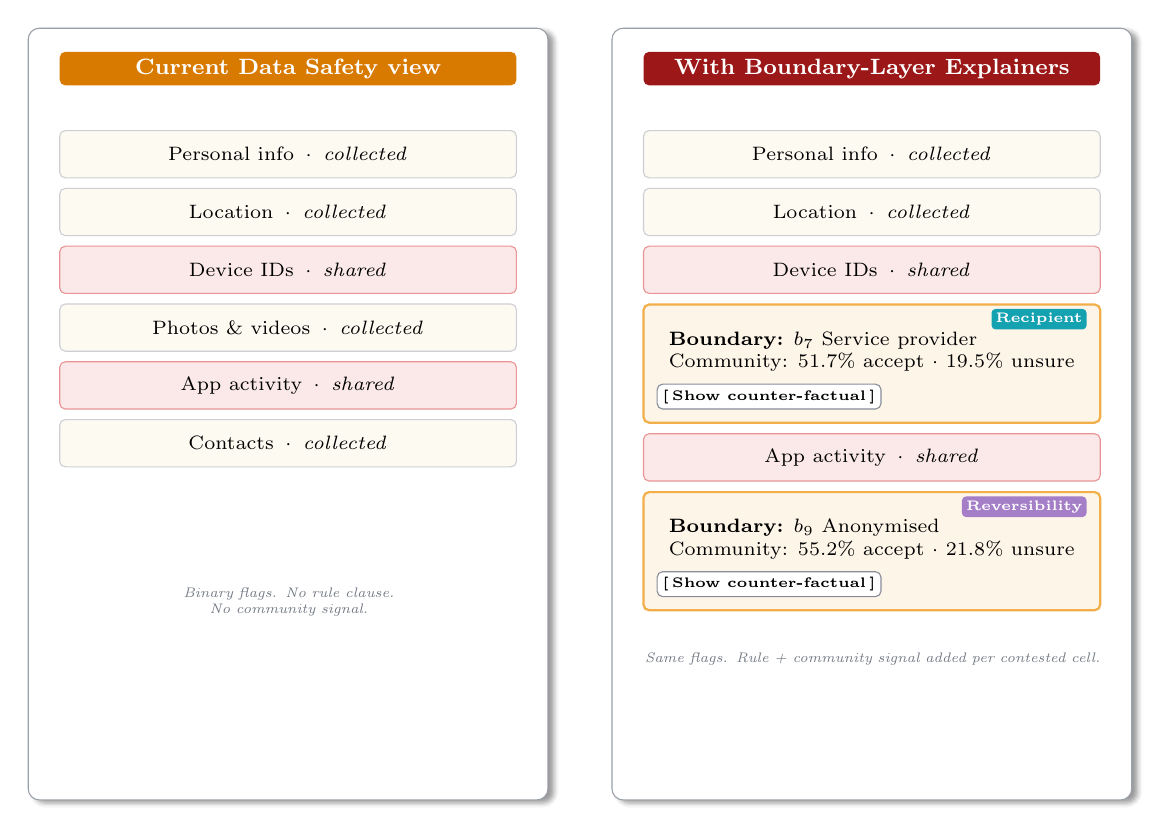
\begin{tikzpicture}[font=\sffamily,
  panel/.style={draw=bmInk!50,rounded corners=4pt,fill=white,
                minimum width=66mm,minimum height=98mm,anchor=north,
                blur shadow={shadow blur steps=4,shadow yshift=-0.4mm}},
  header/.style={font=\footnotesize\bfseries,text=white,
                 rounded corners=2pt,inner sep=2.5pt,
                 minimum width=58mm,anchor=north,align=center},
  rownorm/.style={draw=bmInk!25,rounded corners=2pt,fill=bmCream!60,
              font=\scriptsize,minimum width=58mm,minimum height=6mm,
              anchor=north,align=left,inner sep=1.8mm},
  rowflag/.style={draw=bmRed!50,rounded corners=2pt,fill=bmRed!10,
              font=\scriptsize,minimum width=58mm,minimum height=6mm,
              anchor=north,align=left,inner sep=1.8mm},
  drawer/.style={draw=bmAmber!85,thick,rounded corners=2pt,fill=bmAmber!10,
              font=\scriptsize,minimum width=58mm,minimum height=15mm,
              anchor=north,align=left,inner sep=1.8mm},
  pill/.style={rounded corners=1.5pt,inner sep=1.5pt,
               font=\tiny\bfseries,text=white,anchor=east},
  btn/.style={draw=bmInk!60,rounded corners=2pt,fill=white,
              font=\tiny\bfseries,inner sep=2pt}]

% ===== LEFT PANEL: Current view =====
\node[panel,anchor=north west] (L) at (0,0) {};
\node[header,fill=tierLabel!85!black] at ($(L.north)+(0,-3mm)$)
   {Current Data Safety view};
\node[rownorm] (l1) at ($(L.north)+(0,-13mm)$) {Personal info $\,\cdot\,$ \emph{collected}};
\node[rownorm] (l2) at ($(l1.south)+(0,-1.2mm)$) {Location $\,\cdot\,$ \emph{collected}};
\node[rowflag] (l3) at ($(l2.south)+(0,-1.2mm)$) {Device IDs $\,\cdot\,$ \emph{shared}};
\node[rownorm] (l4) at ($(l3.south)+(0,-1.2mm)$) {Photos \& videos $\,\cdot\,$ \emph{collected}};
\node[rowflag] (l5) at ($(l4.south)+(0,-1.2mm)$) {App activity $\,\cdot\,$ \emph{shared}};
\node[rownorm] (l6) at ($(l5.south)+(0,-1.2mm)$) {Contacts $\,\cdot\,$ \emph{collected}};
\node[font=\tiny\itshape,align=center,anchor=north,text=bmInk!70,
      text width=58mm,below=14mm of l6]
   {Binary flags. No rule clause.\\ No community signal.};

% ===== RIGHT PANEL: BLE-enhanced =====
\node[panel,anchor=north west] (R) at ($(L.north east)+(8mm,0)$) {};
\node[header,fill=tierUser!85!black] at ($(R.north)+(0,-3mm)$)
   {With Boundary-Layer Explainers};
\node[rownorm] (r1) at ($(R.north)+(0,-13mm)$) {Personal info $\,\cdot\,$ \emph{collected}};
\node[rownorm] (r2) at ($(r1.south)+(0,-1.2mm)$) {Location $\,\cdot\,$ \emph{collected}};
\node[rowflag] (r3) at ($(r2.south)+(0,-1.2mm)$) {Device IDs $\,\cdot\,$ \emph{shared}};
\node[drawer]  (d3) at ($(r3.south)+(0,-1.2mm)$)
   {\textbf{Boundary:} $b_7$ Service provider \\
    Community: 51.7\% accept $\cdot$ 19.5\% unsure\\[2pt]};
% pill + button overlaid on drawer
\node[pill,fill=bmTeal!85!black] at ($(d3.north east)+(-1.8mm,-2mm)$) {Recipient};
\node[btn,anchor=south west] at ($(d3.south west)+(1.8mm,1.8mm)$) {[\,Show counter-factual\,]};

\node[rowflag] (r5) at ($(d3.south)+(0,-1.2mm)$) {App activity $\,\cdot\,$ \emph{shared}};
\node[drawer]  (d5) at ($(r5.south)+(0,-1.2mm)$)
   {\textbf{Boundary:} $b_9$ Anonymised \\
    Community: 55.2\% accept $\cdot$ 21.8\% unsure\\[2pt]};
\node[pill,fill=bmPurple!85] at ($(d5.north east)+(-1.8mm,-2mm)$) {Reversibility};
\node[btn,anchor=south west] at ($(d5.south west)+(1.8mm,1.8mm)$) {[\,Show counter-factual\,]};

\node[font=\tiny\itshape,align=center,anchor=north,text=bmInk!70,
      text width=58mm,below=4mm of d5]
   {Same flags. Rule + community signal added per contested cell.};
\end{tikzpicture}
\caption{A worked side-by-side mock-up of the Data Safety section for
a fictional social app (\textsc{SocialNova}) under the current
renderer (left) and a BLE-enhanced renderer (right). The right panel
adds, per contested cell, the boundary case the policy applied, the
community-accepted rate, and a one-tap counter-factual toggle. The
unflagged categories remain collapsed to preserve scannability.}
\label{fig:mockup}
\end{figure}


The mock-up illustrates two design decisions explicitly. \emph{First},
not every cell carries a drawer: \textsc{personal information}
collected and \textsc{location} collected pass through without a
drawer because they are not the product of a contested boundary
case. The drawers appear on the cells that \emph{are} the product
of a contested case --- \textsc{Device IDs} shared via service
provider ($b_7$) and \textsc{App activity} shared via anonymised
analytics ($b_9$). \emph{Second}, the unflagged categories remain
collapsed by default, preserving the scannability that
nutrition-style labels were designed for. A user who only wants the
binary summary still gets it; a user who wants to interrogate a
flag has the inference layer one tap away. This dual-mode behaviour
is, in our reading, the operational meaning of ``treat the user as
the audience of an inference, not the consumer of a fact''.

A potential objection is that a 310-app corpus across one app
category cannot, by itself, calibrate the community signal for the
entire Play Store. We agree. The community signal in our mock-up
is calibrated against the survey reported in this paper; a deployed
BLE renderer would re-estimate the signal continuously against
the platform's own opt-in label-browsing telemetry. The methodology
is the same; only the data source changes.

\subsection{Architectural sketch}\label{sec:arch}

A two-layer Data Safety renderer keeps the existing summary view
unchanged at \emph{Layer~1} and adds an expandable BLE drawer per
category--purpose cell at \emph{Layer~2}. Layer~1 is what Google
Play ships today; the developer declaration drives it, and our
proposal does not alter either the data the developer provides or
the way that data is summarised. Layer~2 is new: it consumes the
same declaration, looks up which boundary case the developer
claimed in the Console, and renders a drawer with the rule clause,
the community signal, and the counter-factual toggle. Layer~3 is
the toggle itself, which re-renders the flag under the negation of
the claimed boundary predicate.

% Figure: two-layer architectural sketch — labels OUTSIDE boxes so they
% never collide with content; arrows are single straight lines.
\begin{figure}[!htbp]
\centering
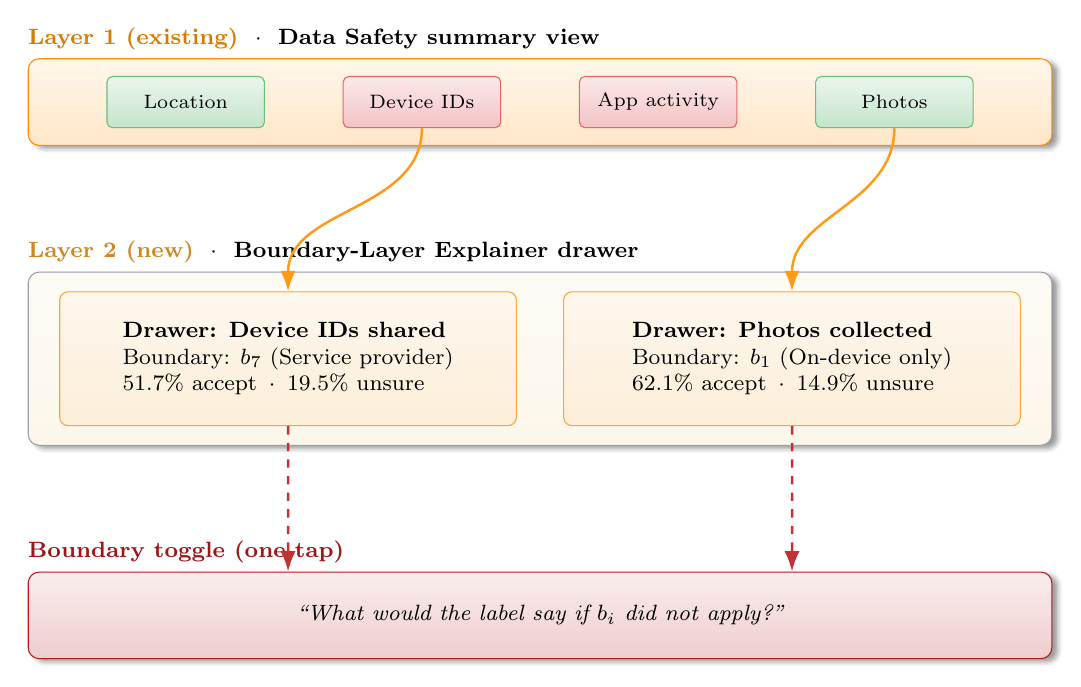
\begin{tikzpicture}[font=\sffamily,
  layerbox/.style={draw=bmInk,rounded corners=4pt,minimum width=130mm,
                   inner sep=2.5mm,
                   blur shadow={shadow blur steps=4,shadow yshift=-0.4mm}},
  layerlbl/.style={font=\footnotesize\bfseries,anchor=south west,inner sep=0pt},
  drawer/.style={draw=bmAmber!90,rounded corners=3pt,fill=white,
                 minimum width=58mm,minimum height=17mm,
                 font=\footnotesize,align=left,inner sep=2.2mm,
                 anchor=center},
  cellG/.style={draw=bmGreen!70,rounded corners=2pt,top color=bmGreen!10,
                bottom color=bmGreen!28,minimum width=20mm,minimum height=6.5mm,
                font=\scriptsize,anchor=center},
  cellR/.style={draw=bmRed!70,rounded corners=2pt,top color=bmRed!10,
                bottom color=bmRed!28,minimum width=20mm,minimum height=6.5mm,
                font=\scriptsize,anchor=center},
  arr/.style={-{Latex[length=2.6mm]},line width=0.9pt,draw=bmInk!85}]

% ===== LAYER 1 — label above, box below =====
\node[layerlbl] (lb1) at (-6.5,5) {\textcolor{tierLabel!85!black}{Layer 1 (existing)} \;$\cdot$\; Data Safety summary view};
\node[layerbox,top color=tierLabel!8,bottom color=tierLabel!22,draw=tierLabel,
      anchor=north west,minimum height=11mm] (L1) at ($(lb1.south west)+(0,-1mm)$) {};
% Cells inside L1
\node[cellG] at ($(L1.center)+(-4.5,0)$) {Location};
\node[cellR] (cB) at ($(L1.center)+(-1.5,0)$) {Device IDs};
\node[cellR] at ($(L1.center)+(1.5,0)$)  {App activity};
\node[cellG] (cD) at ($(L1.center)+(4.5,0)$) {Photos};

% ===== LAYER 2 — label above, box below containing drawers =====
\node[layerlbl,anchor=north west] at ($(L1.south west)+(0,-12mm)$)
   (lb2) {\textcolor{bmAmber!85!black}{Layer 2 (new)} \;$\cdot$\; Boundary-Layer Explainer drawer};
\node[layerbox,top color=bmCream!50,bottom color=bmCream,draw=bmInk!50,
      anchor=north west,minimum height=22mm] (L2) at ($(lb2.south west)+(0,-1mm)$) {};
% Two drawers inside L2, side by side, in the center
\node[drawer,top color=bmAmber!8,bottom color=bmAmber!18] (d1)
   at ($(L2.center)+(-3.2,0)$)
   {\textbf{Drawer: Device IDs shared}\\
    Boundary: $b_7$ (Service provider)\\
    51.7\% accept $\,\cdot\,$ 19.5\% unsure};
\node[drawer,top color=bmAmber!8,bottom color=bmAmber!18] (d2)
   at ($(L2.center)+(3.2,0)$)
   {\textbf{Drawer: Photos collected}\\
    Boundary: $b_1$ (On-device only)\\
    62.1\% accept $\,\cdot\,$ 14.9\% unsure};

% Arrows from cells (L1) to drawers (L2)
\draw[arr,draw=tierLabel!90] (cB.south) to[out=-90,in=90] (d1.north);
\draw[arr,draw=tierLabel!90] (cD.south) to[out=-90,in=90] (d2.north);

% ===== LAYER 3 — toggle box =====
\node[layerlbl,anchor=north west] at ($(L2.south west)+(0,-12mm)$)
   (lb3) {\textcolor{tierUser!85!black}{Boundary toggle (one-tap)}};
\node[layerbox,top color=tierUser!8,bottom color=tierUser!22,draw=tierUser,
      anchor=north west,minimum height=11mm] (L3) at ($(lb3.south west)+(0,-1mm)$) {};
\node[font=\footnotesize\itshape,align=center] at (L3.center)
   {``What would the label say if $b_i$ did not apply?''};

% Arrows from drawers down to L3
\draw[arr,draw=tierUser!90,dashed] (d1.south) to[out=-90,in=90] ($(L3.north)+(-32mm,0)$);
\draw[arr,draw=tierUser!90,dashed] (d2.south) to[out=-90,in=90] ($(L3.north)+(32mm,0)$);
\end{tikzpicture}
\caption{Architectural sketch of a two-layer Data Safety renderer.
Each layer has its title rendered \emph{above} its box so the title
never collides with content. Layer~1 (top) is the unchanged Data
Safety summary view that Google Play already ships. Layer~2 (middle)
hosts a per-cell drawer that surfaces the boundary case which
produced the cell value and the community signal estimated from our
data. The boundary toggle (bottom) re-renders the flag under the
counter-factual that the boundary case did not apply, giving the
user a one-tap view of the inference rule's effect on the visible
label.}
\label{fig:two-layer-arch}
\end{figure}


Figure~\ref{fig:two-layer-arch} sketches the component graph. The
implementation cost is low for three reasons. First, the platform
\emph{already} knows which boundary case the developer claimed: the
developer ticks the corresponding exception in the Console when
filing the Data Safety declaration. Surfacing that selection on the
user-side simply makes visible information that is already collected
on the developer-side. Second, the community signal can be computed
centrally from existing telemetry on label browsing; nothing about
the developer workflow needs to change. Third, the counter-factual
toggle is a single Boolean substitution against
Eq.~\ref{eq:policy}: the renderer computes the flag the label
\emph{would} have shown if the developer's claimed boundary case
had not applied. This is a pure function of the declaration plus
the negated predicate.

The architectural decision we want to highlight is \emph{separation
of concerns}. The policy-layer rule (Eq.~\ref{eq:policy}) remains
the source of truth for what the flag is; the user-layer drawer
(Layer~2) communicates how the rule was applied and how widely
accepted it is. Decoupling these two responsibilities means that
changes to platform policy --- adding a tenth boundary case, for
example --- propagate to the drawer without touching the summary
renderer, and that updates to the community signal (as more users
browse labels) propagate without touching either.

\subsection{Five untested design implications}\label{sec:implications}

Building on the typology, the quantification, and the BLE pattern,
we extract five design implications for the next generation of
app-store privacy labels. We do not claim these as confirmed by a
deployed study; they are formulated to be \emph{falsifiable} in a
between-subjects label experiment, and we describe the falsification
protocol for each. The implications are ordered from
the most architectural to the most fine-grained.

\paragraph{Implication 1: Surface the boundary, not just the
outcome.} The single most basic move is to render the boundary
case the policy applied alongside the cell value. Our data give a
direct prediction: presenting the boundary case should reduce the
gap between the user's installation behaviour and their stated
preferences on Type~B (recipient) cases more than on Type~A
(reversibility) cases, because recipient information is the
content the user is asking for and is missing from the current
label. The falsifier is a between-subjects experiment that crosses
``BLE drawer present / absent'' with ``boundary case is Type A /
B / C'' and measures installation intent against post-explanation
preference.

\paragraph{Implication 2: Express the boundary in consequence-first
language.} The same boundary case can be rendered as a policy
clause (``transfer to a service provider acting on the developer's
behalf'') or as a user consequence (``passes \{Device IDs\} to a
contracted processor''). Our rationale coding shows that users
reach spontaneously for the second formulation. The falsifier
crosses the rule clause's language (policy-first vs.
consequence-first) on otherwise identical drawers; the prediction
is that the consequence-first wording produces both higher recall
of the underlying rule and a smaller Yes--Maybe gap than the
policy-first wording.

\paragraph{Implication 3: Signal community uncertainty alongside
agreement.} A single community percentage (``$X\%$ accept'') is the
naive rendering and the wrong one. Our data show that the
trichotomy is informative: a $61.8\%$ Yes / $38.2\%$ Maybe
distribution ($b_3$ off-device ephemeral) is qualitatively different
from a $61.8\%$ Yes / $0\%$ Maybe / $38.2\%$ No distribution, and
only the first indicates the kind of disagreement the BLE is
designed to expose.
The falsifier renders the same Yes-rate as either ``$X\%$ accept''
or ``$X\%$ accept, $Y\%$ unsure'' and measures whether users on
the second condition are more likely to open the boundary toggle.

\paragraph{Implication 4: Make the alternative one tap away.} The
boundary toggle is the design move that distinguishes a BLE from a
tooltip. The hypothesis is that users want to know, concretely,
what the label \emph{would have} said had the boundary case not
applied, and that without that affordance the BLE drawer degrades
to a wordy tooltip. The falsifier compares a drawer-with-toggle
condition to a drawer-without-toggle condition on
boundary-case-comprehension and installation behaviour.

\paragraph{Implication 5: Treat ``Maybe'' as a first-class state.}
Both the user instrument and the BLE community signal carry a
three-valued response. Collapsing that into a binary at any point
loses information that our data show is structurally informative.
The falsifier renders the BLE community signal either as a
two-valued bar (Yes\,/\,not-Yes) or a three-valued bar
(Yes\,/\,Maybe\,/\,No) and measures whether the three-valued
condition produces more accurate user predictions of the
underlying disagreement.

The five implications together specify a complete experimental
programme rather than a single intervention. Each implication
contributes a separable factor whose effect can be measured against
an installation-intent outcome. A reader who is sceptical of any
single implication can dis-confirm it independently; this is, we
think, the appropriate standard for a measurement-led HCI design
contribution.

%==========================================================================
\section{A pre-registered evaluation plan for the BLE pattern}
\label{sec:eval-plan}

The measurement contribution of this paper does not by itself test
the BLE pattern. We have specified, and pre-registered before any
data collection, a mixed-method evaluation that is built into the
manuscript's supplementary materials. The plan combines an online
vignette experiment with a small in-lab think-aloud arm and is
designed to be falsifiable on each of the five design
implications of Sec.~\ref{sec:implications}.

\paragraph{Quantitative arm.}
A between-subjects vignette experiment compares the current Data
Safety renderer against the BLE-enhanced renderer on a fictional
app pool. Each participant sees four apps sampled by
stratification from a 12-app pool, guaranteeing at least one app
from each of the Reversibility / Recipient / Consent families.
The pre-registered primary outcome is boundary-case comprehension
(MCQ on the boundary case applied); secondary outcomes are
perceived label accuracy, perceived comprehensiveness, and an
equivalence test on installation intent. Target $N{=}200$
(Prolific), powered for a medium effect ($d{=}0.40$, $\alpha{=}0.05$,
power $0.80$). Pre-specified exclusions cover attention-check
failure, completion-time floors, and straight-lining.

\paragraph{Qualitative arm.}
A think-aloud study with 12--15 participants triangulates the
quantitative findings with fine-grained evidence on how users open
and reason about the BLE drawers. The coding book is structured
around four axes (drawer affordance, rule clause, community signal,
decision moment) with seventeen codes; the calibration target is
Cohen's $\kappa \geq 0.70$ per code on a 20\% sample.

\paragraph{Hypothesis structure.}
Five hypotheses are pre-registered with explicit
\emph{supported / refuted / no decision} decision rules, including
a TOST equivalence test for the null prediction that installation
intent does not differ between conditions. The complete
pre-registration, the analysis pipeline, the consent and recruitment
text, and a working browser-based prototype of the BLE renderer
are released in the \texttt{UserStudy/} folder of the supplementary
material. Section~7 of the manuscript will, on revision, report
the results of this evaluation; the present paper is the measurement
prerequisite.

%==========================================================================
\section{Discussion and Limitations}\label{sec:discussion}

\paragraph{Honesty is not enough.}
Audits of Apple and Google labels make the now-familiar point that
declarations frequently understate observed
behaviour~\citep{koch:etal:2022,kollnig:etal:2022,
bhagavatula:etal:2023,khandelwal:etal:2023}. Our data add the
converse: even when declarations are honest \emph{at the policy
layer}, they fail to be honest \emph{at the user layer} for a
substantial share of users on every boundary case we tested. A
redesigned label that closes the honesty gap does not automatically
close the disclosure gap; a redesign must also close the
boundary-case mismatch.

\paragraph{Why we do not propose removing boundary cases.}
A natural reaction is to argue that boundary cases should be
eliminated and every off-device transfer reported, full stop. We
resist this. Boundary cases exist for principled reasons:
anonymisation, ephemeral processing, and service-provider contracts
are real privacy-engineering practices, not legal fictions. The HCI
problem is not that the boundary case exists; it is that the user is
not told which boundary case was applied. The BLE pattern preserves
the policy semantics and adds the missing inference layer.

\paragraph{Relation to contextual integrity.}
In CI terms~\citep{nissenbaum:2004,nissenbaum:2010,barth:etal:2006},
the boundary-case mismatch is a clash between the
\emph{transmission principle} the platform encodes (``it is
appropriate to share for legal purposes'') and the principle the
user holds (``it depends on the law''). The BLE pattern surfaces the
transmission principle next to the flag, giving users the
information CI says they need to assess
appropriateness~\citep{shvartzshnaider:etal:2019,apthorpe:etal:2018,
martin:nissenbaum:2017}.

\paragraph{Implications for regulators and platforms.}
The boundary-case mismatch has two regulatory readings. The
narrower: the binary flag is inadequate as a basis for meaningful
consent under data-minimisation regimes such as the
GDPR~\citep{gdpr:2016}. The wider: the next generation of disclosure
schemes ought to surface the inference layer by default, not as a
tooltip on hover. We do not propose that the platform classify
boundary-case mismatches as policy violations --- this would penalise
honest developers --- but that the platform render the boundary case,
the community signal, and the counter-factual as standard parts of
the disclosure.

\paragraph{Implications for developers.}
Interview audits~\citep{bhagavatula:etal:2023,khandelwal:etal:2023,
li:etal:2022} report that developers themselves struggle with the
boundary-case definitions. The mismatch we measure on the user side
is mirrored on the developer side. A BLE renderer would make the
boundary case the developer chose visible to every label viewer,
which we expect to push declaration behaviour toward conservative
reporting.

\paragraph{Implications for HCI research.}
The boundary-case mismatch is a particular instance of a more
general problem: the user interface for a classifier hides the
classifier. Recommendation, content-moderation, ad-relevance, and
credit-scoring interfaces all share this structure with the privacy
label. The two-layer accuracy framework is transportable to each.

\paragraph{Limitations.}
The 87-participant crowd-work sample is modest and skews toward
English-speaking, mobile-fluent users with internet income. We
propose a design pattern but do not evaluate a deployed prototype;
following the IJHCS tradition of separating measurement and
intervention contributions, we treat the empirical pattern as the
contribution of this paper. The instrument is cross-sectional;
mental models of privacy evolve with
events~\citep{rader:etal:2012,wash:rader:2015,sannon:etal:2018}. We
restricted to the Social app category to stabilise contextual norms;
the mismatch may take different shapes in other categories. Apple's
labels have overlapping but not identical boundary cases, and
between-platform replication is the obvious follow-up. The precision
analysis confirms that $N{=}87$ is sufficient to detect the
boundary-case mismatch reliably, but not large enough for
fine-grained between-population comparisons.

\paragraph{Future work.}
Three follow-up studies are obvious. (i) A between-subjects label
experiment comparing the current Data Safety renderer to a
BLE-enhanced renderer, with installation intent and post-install
behaviour as outcomes. (ii) Cross-platform replication to Apple's
label and to emerging non-US schemes. (iii) A diary study of how
boundary-case signalling interacts with daily app use rather than
one-shot install decisions.

%==========================================================================
\section{Conclusion}\label{sec:conclusion}

App-store privacy labels are conventionally read as a description of
fact. We have argued they are better read as the \emph{output of an
inference rule}: the flag appears, or fails to appear, because a
policy boundary case decided the underlying practice was, or was
not, the kind of thing the user needs to be told about. When the
platform and the user disagree about the boundary case, the label
can be ``accurate'' in policy terms and ``wrong'' in user terms. We
measured this gap in an 87-participant survey across Google Play's
nine boundary cases and found that the soft mismatch lies between
$16.7\%$ ($b_2$ E2E encryption) and $38.2\%$ ($b_3$ off-device
ephemeral processing), with the Maybe rate exceeding $16\%$ on
every case. We named the phenomenon the \emph{boundary-case
mismatch}, gave a two-layer accuracy framework, and proposed a
falsifiable design pattern --- the \emph{Boundary-Layer Explainer}
--- that surfaces the inference rule without disturbing the policy
semantics that produced it. A pre-registered mixed-method
evaluation of the pattern is specified in Sec.~\ref{sec:eval-plan}
and is the subject of the companion paper.

%==========================================================================
% IJHCS REQUIRED back matter
%==========================================================================
\section*{CRediT author statement}
\noindent\emph{Anonymised for review.} A CRediT
(Contributor Roles Taxonomy) breakdown of conceptualisation,
methodology, formal analysis, investigation, writing -- original
draft, writing -- review \& editing, supervision, and project
administration will be provided in the camera-ready manuscript.

\section*{Declaration of competing interest}
The authors declare that they have no known competing financial
interests or personal relationships that could have appeared to
influence the work reported in this paper.

\section*{Funding}
\emph{Anonymised for review.} A complete funding statement will be
provided in the camera-ready manuscript.

\section*{Data and code availability}
The de-identified survey export, free-text rationales, coding book,
and the Python replication notebook (\texttt{boundary\_cases.ipynb})
are released as supplementary material alongside the paper. The
notebook regenerates every numeric value, table, and figure in this
manuscript from the raw export. The 310-app corpus and the
participant--app pairing matrix are released as CSV files.

\section*{Ethics statement}
The protocol was approved by the principal authors' institutional
research ethics board. Participants gave informed consent at the
start of the survey and were paid USD~\$3 for a median completion
time of 22 minutes. Identifiers (email addresses collected by the
crowd-work platform for payment) were removed prior to analysis and
do not appear in any released material.

\section*{Acknowledgments}
\emph{Anonymised for review.}

\bibliography{references}

\appendix

\section{Instrument: full text (selected items)}\label{app:instrument}
The full survey instrument is in supplementary material~S1. For
self-containment we reproduce the wording of the nine boundary-case
items that are the focus of this paper.

\subsection*{Part III: Collection boundary cases}
\textit{``Below are situations involving an Android app and your
data. For each, indicate whether the situation should \textbf{not}
be counted as the app collecting your data. Use Yes / No / Maybe and
add a one-line reason.''}
\begin{enumerate}
\item[$b_1$.] ``An app accesses the data only on your device and it
is not sent off your device.''
\item[$b_2$.] ``Your data is sent off the device using end-to-end
encryption.''
\item[$b_3$.] ``Your data is sent off the device but only processed
ephemerally.''
\item[$b_4$.] ``The app may redirect you to a different service to
complete a certain action.''
\end{enumerate}

\subsection*{Part IV: Sharing boundary cases}
\textit{``Below are situations in which an Android app transfers
your data to someone else. For each, indicate whether the situation
should \textbf{not} be counted as the app sharing your data. Use
Yes / No / Maybe and add a one-line reason.''}
\begin{enumerate}
\item[$b_5$.] ``The data is transferred to a third party based on a
specific action you initiate, where you reasonably expect the data
to be shared.''
\item[$b_6$.] ``The data transfer to a third party is prominently
disclosed in the app, and the app requests your consent in a way
that meets the requirements of Google Play's User Data policy.''
\item[$b_7$.] ``The data is transferred to a service provider to
process it on the developer's behalf.''
\item[$b_8$.] ``The data is transferred for specific legal
purposes.''
\item[$b_9$.] ``The data transferred is fully anonymised so it can
no longer be associated with any individual.''
\end{enumerate}

\section{App corpus and pairing matrix}\label{app:corpus}
The 310-app corpus, sampling weights, and per-participant pairing
matrix are in supplementary material~S2.

\section{Replication notebook}\label{app:replication}
The Python notebook \texttt{boundary\_cases.ipynb} regenerates every
numeric value reported in this paper from the raw de-identified
survey export. The notebook is split into three sections mirroring
the paper structure: (i) per-category personalness and per-purpose
acceptance from the aggregate file; (ii) per-boundary-case Yes /
Maybe distributions with Wilson 95\% confidence intervals;
(iii) per-category app-instance necessity, with within-person
stratification by the participant's Yes/Maybe classification of the
category.

\section{Materials for the planned BLE evaluation}\label{app:eval}
The \texttt{UserStudy/} folder of the supplementary material contains
the working browser-based prototype (Conditions A/B), the
12-app fictional pool (with per-participant deterministic
stratified sampling), the pre-registered protocol and instrument
for the vignette experiment, the moderator protocol and coding book
for the think-aloud sessions, and the analysis pipeline that
implements the five pre-registered hypotheses with
\emph{supported / refuted / no decision} decision rules.

\end{document}
